%% For submission and review of your manuscript please change the
%% command to \documentclass[manuscript, screen, review]{acmart}.
%%
%% When submitting camera ready or to TAPS, please change the command
%% to \documentclass[sigconf]{acmart} or whichever template is required
%% for your publication.
% table is there because https://tex.stackexchange.com/a/83102 said so.
\documentclass[acmlarge, manuscript, screen, review, anonymous, table]{acmart}

%% \BibTeX command to typeset BibTeX logo in the docs
\AtBeginDocument{%
  \providecommand\BibTeX{{%
    Bib\TeX}}}

%% Rights management information.  This information is sent to you
%% when you complete the rights form.  These commands have SAMPLE
%% values in them; it is your responsibility as an author to replace
%% the commands and values with those provided to you when you
%% complete the rights form.
\setcopyright{acmlicensed}
\copyrightyear{2018}
\acmYear{2018}
\acmDOI{XXXXXXX.XXXXXXX}


%% These commands are for a JOURNAL article.
\acmJournal{POMACS}
\acmVolume{37}
\acmNumber{4}
\acmArticle{111}
\acmMonth{8}

%% Submission ID.
%% Use this when submitting an article to a sponsored event. You'll
%% receive a unique submission ID from the organizers
%% of the event, and this ID should be used as the parameter to this command.
%%\acmSubmissionID{123-A56-BU3}

%% The majority of ACM publications use numbered citations and
%% references.  The command \citestyle{authoryear} switches to the
%% "author year" style.
%%
%% If you are preparing content for an event
%% sponsored by ACM SIGGRAPH, you must use the "author year" style of
%% citations and references.
%% Uncommenting
%% the next command will enable that style.
%%\citestyle{acmauthoryear}


\usepackage{amsmath,amsfonts}
\usepackage{amsthm}
\usepackage{algorithm,algorithmic}  %% typset algorithms
\usepackage{arydshln}
\usepackage [autostyle, english = american]{csquotes}
\usepackage{booktabs}  %% What is this for?
\usepackage{centernot}
\usepackage{graphicx}
\usepackage{listings}
\usepackage{mdframed}
\usepackage{multirow}
\usepackage{newunicodechar}
\usepackage{textcomp}
\usepackage{textgreek}
\usepackage{xcolor}
\usepackage{xspace}

\makeatletter
\newif\ifanonymous
\@ifclasswith{acmart}{anonymous}{\anonymoustrue}{\anonymousfalse}
\makeatother

%https://tex.stackexchange.com/a/169103
\setlength\dashlinedash{0.2pt}
\setlength\dashlinegap{2.0pt}
\setlength\arrayrulewidth{0.3pt}

\lstdefinelanguage{cho}{
    alsoletter={@01},
    sensitive=true,
    basicstyle={\ttfamily},
    morekeywords=[1]{MACRO,AS,ENDMACRO},
    keywordstyle=[1]{\bfseries},
    morekeywords=[2]{SEND,TO,OBLIVIOUSLY,FOR,OUTPUT,SECRET,FLIP},
    keywordstyle=[2]{\bfseries\color{blue}},
    morekeywords=[3]{DO,GET},
    keywordstyle=[3]{\bfseries},
    morekeywords=[4]{XOR,+,<>,!=,AND,*,^,NOT,!,~},
    keywordstyle=[4]{},
    morekeywords=[5]{true,false,0,1},
    keywordstyle=[5]{\color{teal}},
    identifierstyle={\color{violet}},
    morecomment=[l]{--},
    morecomment=[s]{\{-}{-\}},
    commentstyle={\color{gray}},
    numbers={left},
    xleftmargin=20px,
    numberstyle={\color{gray}\itshape},
    numbersep=15px,
}

% use these if you also want π to work in math mode
\newunicodechar{Π}{\ifmmode\Pi\else\textPi\fi}
\newunicodechar{⫫}{\mathrel{\perp\!\!\!\perp}}

% use quotes as smart-quotes. https://tex.stackexchange.com/a/52354
\MakeOuterQuote{"}

%the template suggests we shouldn't do this.
%\renewcommand{\paragraph}[1]{\vspace*{2pt}\noindent\textbf{#1}}

\newcommand{\bigpar}[1]{\left( #1 \right)}
\newcommand{\eg}{\textit{e.g.}\xspace}
\newcommand{\github}{\ifanonymous redacted for anonymous submission\else https://github.com/ShapeOfMatter/dt-sim\fi}
\newcommand{\highlight}[2]{\colorbox{#1}{#2}}
\newcommand{\icONE}[1][cho]{\inlinecode[#1]{1}}
\newcommand{\iczed}[1][cho]{\inlinecode[#1]{0}}
\newcommand{\ie}{\textit{i.e.}\xspace}
\newcommand{\inlinecode}[2][cho]{\lstinline[language=#1]{#2}}
\newcommand{\langname}{\textsc{\textbf{.}CHO}\xspace}
\newcommand{\negquad}{\!\!\!\!}
\newcommand{\STAB}[1]{\begin{tabular}{@{}c@{}}#1\end{tabular}} % https://tex.stackexchange.com/a/416169
\newcommand{\toolname}{\textsc{DT-SIM}\xspace}
\newcommand{\vertvec}[1]{\left\langle { \renewcommand*{\arraystretch}{1}\begin{matrix} #1 \end{matrix} } \right\rangle}

\definecolor{ideal}{rgb}{ 0.8, 1.0, 0.8}
\definecolor{real}{rgb}{  0.8, 0.8, 0.8}
\definecolor{secret}{rgb}{1.0, 0.8, 0.8}
\definecolor{nullmutation}{gray}{0.85}
\definecolor{insecmutation}{gray}{1.00}
\definecolor{correct}{rgb}{  0.80, 1.00, 0.85}
\definecolor{incorrect}{rgb}{1.00, 0.80, 0.85}

\newcommand{\mynote}[2]
    {{\color{red} \fbox{\bfseries\sffamily\scriptsize#1}
    {\small$\blacktriangleright$\textsf{\emph{#2}}$\blacktriangleleft$}}~}
\newcommand{\todo}[1]{\mynote{TODO}{#1}}

%% end of the preamble, start of the body of the document source.
\begin{document}

\title{\toolname: Property-Based Testing for MPC Security}

\author{Mako Bates}
\email{mako.bates@uvm.edu}
\orcid{0009-0001-9933-1728}
\affiliation{%
 \institution{University of Vermont}
 \city{Burlington}
 \state{Vermont}
 \country{US}}
\author{Joseph P. Near}
\email{jnear@uvm.edu}
\orcid{0000-0002-3203-3742}
\affiliation{%
 \institution{University of Vermont}
 \city{Burlington}
 \state{Vermont}
 \country{US}}


%\newtheorem{definition}{Definition}

\newcommand{\termOfArt}[1]{\textbf{#1}}

\begin{abstract}
  Formal methods for guaranteeing that a protocol satisfies a cryptographic security definition have advanced substantially,
  but such methods are labor intensive and the need remains for an automated tool that can positively identify an insecure protocol.
  In this work, we demonstrate that property-based testing, \emph{"run it a bunch of times and see if it breaks"},
  can be an effective strategy for detecting security bugs in secure protocols.
  We specifically target Secure Multi-Party Computation (MPC), because formal methods targeting this security definition for bit-model implementations
  are especially difficult.
  Using results from the literature for Probabilistic Programming Languages and statistical inference,
  we devise \toolname, a test that can
  detect various flaws in a bit-level implementation of an MPC protocol.
  The test is grey-box; it requires only transcripts of randomness consumed by the protocol and of the inputs, outputs, and messages.
  It successfully detects several different mistakes and biases introduced into two different implementations of the classic GMW protocol.
  We also include an analysis of the parameters of the test, and discussion of what makes detection of MPC (in)security difficult.
\end{abstract}

%%
%% The code below is generated by the tool at http://dl.acm.org/ccs.cfm.
%% Please copy and paste the code instead of the example below.
%%
\begin{CCSXML}
<ccs2012>
 <concept>
  <concept_id>00000000.0000000.0000000</concept_id>
  <concept_desc>Do Not Use This Code, Generate the Correct Terms for Your Paper</concept_desc>
  <concept_significance>500</concept_significance>
 </concept>
 <concept>
  <concept_id>00000000.00000000.00000000</concept_id>
  <concept_desc>Do Not Use This Code, Generate the Correct Terms for Your Paper</concept_desc>
  <concept_significance>300</concept_significance>
 </concept>
 <concept>
  <concept_id>00000000.00000000.00000000</concept_id>
  <concept_desc>Do Not Use This Code, Generate the Correct Terms for Your Paper</concept_desc>
  <concept_significance>100</concept_significance>
 </concept>
 <concept>
  <concept_id>00000000.00000000.00000000</concept_id>
  <concept_desc>Do Not Use This Code, Generate the Correct Terms for Your Paper</concept_desc>
  <concept_significance>100</concept_significance>
 </concept>
</ccs2012>
\end{CCSXML}

\ccsdesc[500]{Do Not Use This Code~Generate the Correct Terms for Your Paper}
\ccsdesc[300]{Do Not Use This Code~Generate the Correct Terms for Your Paper}
\ccsdesc{Do Not Use This Code~Generate the Correct Terms for Your Paper}
\ccsdesc[100]{Do Not Use This Code~Generate the Correct Terms for Your Paper}

%%
%% Keywords. The author(s) should pick words that accurately describe
%% the work being presented. Separate the keywords with commas.
\keywords{Do, Not, Us, This, Code, Put, the, Correct, Terms, for,
  Your, Paper}

\received{20 February 2007}
\received[revised]{12 March 2009}
\received[accepted]{5 June 2009}

\maketitle

\todo{ACM subjects and keywords.}\\
\todo{add "Description" tags to all tables.}\\
\todo{rewrite appendix A to make enough sense.}\\
\todo{rewrite appendis B to make sense, cover whatever we say it covers, and look nice.}\\



\section{Introduction}

Secure multiparty computation (MPC) protocols~\cite{evans2018pragmatic} allow a group of mutually distrusting parties to compute a shared function over distributed data without revealing that data to each other.
The security of MPC protocols is often expressed as a negation,
\eg secret information should \emph{never} be derivable from an adversary's observations of the system.
Unfortunately, testing generally provides limited evidence that the system is actually secure in the intended ways.
Formal proofs of security are effective, but are tedious to construct and require significant expertise.
As a result:
%
\begin{itemize}
\item Most implementations of MPC protocols are not formally verified.
\item Formal verification tools are challenging to use, and engineers can waste significant time trying to prove properties of insecure implementations.
\item Even for formally-verified software, we would like to have sanity checks
  that protocol implementations actually have the security properties their constituent source-code claims to be proven to have.
\end{itemize}

We present \toolname, an \emph{automatic}, \emph{property-based testing} tool for MPC security. \toolname works by running the protocol thousands of times, then using a statistical independence test to detect security bugs. Our approach is motivated by the success of property-based testing (via tools like \textsc{QuickCheck}) as an approach for finding bugs in software~\cite{fink1997property, claessen2000quickcheck, paraskevopoulou2015foundational}. Unlike previous applications of property-based testing, however, \toolname attempts to falsify a \emph{probabilistic hyperproperty} of the target protocol---a much more challenging setting.

\toolname works by defining security in terms of conditional independence, then performing a statistical test which attempts to falsify this conditional independence property. In MPC protocols, the inputs of the honest parties should be independent of the \emph{views} (\ie the observed message values) of the corrupt parties, conditioned on the protocol's output. Conditioning on the protocol's output is vital for the security definition, since it allows the protocol to \emph{intentionally} leak some information about the inputs via the output---as nearly all MPC protocols do. Manual security proofs for MPC protocols demonstrate this conditional independence property by constructing a \emph{simulator} that ``fakes'' the corrupt parties' views using only the protocol's output.

This formulation of security as conditional independence puts MPC security out of reach of all automated verification tools (and many manual ones). While automated tools have been used to verify security in cryptographic protocols~\cite{gancher2023owl, barthe2019probabilistic, darais2019language, fournet2011information}  (\eg key exchange protocols), these tools are limited to protocols whose \emph{outputs reveal nothing} to the adversary. They are capable of showing independence, but not the kind of \emph{conditional} independence required for MPC security. Recent manual approaches could be used to verify MPC security~\cite{li2023lilac, gancher2023core, haagh2018computer}, but require manual proof.

\toolname is designed to fill the same role as tools like \textsc{QuickCheck}: it can be used to quickly and automatically detect many classes of bugs in MPC protocol implementations, without investing the user's time in a manual security proof.
Using \toolname requires only that key runtime values can be captured during program execution;
it's agnostic to the language and many other details about the subject program.
We have implemented \toolname and tested it empirically on several real-world MPC protocols and on hundreds of randomly-generated protocols; our experimental results suggest that \toolname is capable of scaling to realistic protocols and detecting many security bugs, despite the challenging setting.


\paragraph{Contributions.}
In summary, our contributions are:
%
\begin{itemize}
\item We show how to define MPC security in terms of conditional independence, enabling the use of independence testing tools for checking MPC security.
\item We introduce \toolname, the first property-based testing tool for MPC security.
\item We conduct an empirical evaluation of \toolname, demonstrating its ability to scale to realistic MPC protocols and detect security bugs.
\end{itemize}



\section{Background}

\subsection{MPC security}

Secure Multi-Party Computation (MPC or SMPC, depending on the text)
is a cryptographic process that allows some group of participating parties or machines
to compute a function that depends on all of their private inputs,
without any of them learning anything except the final result\footnote{
    It is possible for each party to have a distinct final result.
}.
Implementations that work on arbitrary functions (representable as circuit computations in some field)
have existed since 1986~\cite{yao1986generate}, % https://ieeexplore.ieee.org/document/4568207
but their use by the public is limited by their performance.
Some performance limitations are fundamental to the problem
(roughly, every branch of the computation must be executed so that the control-flow does not itself leak information),
but techniques have been found to improve performance somewhat.

The traditional expression of MPC assumes a pre-determined function $F$, the \emph{functionality},
mapping the tuple of all participants' input vectors to the respective tuple of output vectors
(or to distributions of outputs, if $F$ is non-deterministic).
For example, Protocol~\ref{fig:example-vac-secure} implements the following function:
$$F_3\bigpar{\mathtt{sec}, \mathtt{pub}}
  := \mathtt{sec} \neq \mathtt{pub}$$
For full formality, $F_3$ would be written as a function from two vectors to two vectors, because there are two parties involved.
\inlinecode{H} provides one input vector containing just \inlinecode{sec},
and \inlinecode{C} provides the other input vector containing just \inlinecode{pub}.
In this example the two parties' output vectors would be the same, containing just the value of \inlinecode{x}.

In an \termOfArt{ideal world}, a trusted third party (the \termOfArt{ideal functionality}) would accept input messages
from all other parties, compute $F$, and then send the parties their respective outputs.
The ideal functionality $F_1$ implemented by Protocol~\ref{fig:example-insecure}
could be reasonably implemented by just declaring a coin from someone's pocket to be the \textit{"trusted third party"},
and ascribing \inlinecode{true} and \inlinecode{false} to heads and tails.
A \termOfArt{real world} protocol $Π$ is said to \emph{correctly} implement $F$ if, for all possible inputs,
$Π$ results in all parties getting the same outputs as they would have in the ideal
world\footnote{In the case of a nondeterministic functionality like $F_1$, the parties get outputs sampled from the correct distribution.}.

The \emph{security} of $Π$ is expressed in terms of a particular threat model and the participants' \textit{"views"}.
For a given functionality $F$, list of parties' inputs $\vec{x}$, and list of parties' outputs $\vec{y}=F(\vec{x})$,
the \termOfArt{ideal world view}, $\mathsf{Ideal}_P(F,\vec{x})$, of a party $P$ is what it sees when running $F$ in the ideal world:
just its inputs $\vec{x}_P$ and its outputs $\vec{y}_P$.
For example, \inlinecode{C}'s ideal world view of an execution of Protocol~\ref{fig:example-vac-protocol}
would be a single random bit, the value of \inlinecode{x} in that execution.
The \termOfArt{real world view}, $\mathsf{Real}_P(Π, \vec{x})$, of a party $P$ is everything it sees while executing its part of $Π$ in the real world:
its inputs, outputs, all messages it receives, and all the bits of random tape it uses.
Continuing the example of Protocol~\ref{fig:example-vac-protocol}, \inlinecode{C}'s real world view would additionally contain
the (independent) random value \inlinecode{_un}
(and technically a duplicate of \inlinecode{x}, because it's both output and a received message).
Both kinds of views extend naturally to lists of parties.

\begin{figure}[tbhp]
  \begin{mdframed}
      \lstinputlisting[language=cho]{insecure.cho}
  \end{mdframed}
  %\newcommand{\gsize}{.38\textwidth}
    \caption{An example protocol, Protocol~\ref{fig:example-insecure}, written in \langname.
    This protocol does \emph{not} demonstrate MPC security.
    It's ideal functionality is \textit{"flip a coin"},
    because the one-bit output is uniformly distributed regardless of anyone's \inlinecode{SECRET}s.}
  \label{fig:example-insecure}
\end{figure}
\begin{figure}[tbhp]
  \begin{mdframed}
      \lstinputlisting[language=cho]{vac_protocol.cho}
  \end{mdframed}
  %\newcommand{\gsize}{.38\textwidth}
  \caption{An example protocol, Protocol~\ref{fig:example-vac-protocol}, written in \langname.
    This protocol \emph{does} demonstrate MPC security, although it's ideal functionality is just \textit{"flip a coin"}.}
  \label{fig:example-vac-protocol}
\end{figure}
\begin{figure}[tbhp]
  \begin{mdframed}
      \lstinputlisting[language=cho]{vac_secure.cho}
  \end{mdframed}
  %\newcommand{\gsize}{.38\textwidth}
  \caption{An example protocol, Protocol~\ref{fig:example-vac-secure} written in \langname.
    This protocol \emph{does} demonstrate MPC security,
    although such security is vacuous because \inlinecode{C} could compute \inlinecode{H}'s \inlinecode{SECRET}
    from the ideal functionality: \textit{"return the xor of the secret and public values"}.}
  \label{fig:example-vac-secure}
\end{figure}



\termOfArt{Passive security}
supposes a computationally-bounded adversary
that can see everything happening inside a fixed subset of the participating machines.
This passive adversary cannot cause the parties to deviate from the protocol $Π$ in any way;
we are interested in whether it can learn anything \emph{beyond} the outputs of the \termOfArt{corrupted} machines
by observing the execution of $Π$.
As an example, this notion of security might be of interest if Alice trusted Bob to participate
in a distributed computation with her, but did not trust him to properly store or destroy the log-files
generated.

\begin{definition}[Passive MPC Security]\label{def:passive-mpc}
  \begin{samepage}
    A protocol $Π$,
    involving participating parties $P$,
    that correctly implements functionality $F$,
    is secure against a passive adversary controlling $C \subset P$ iff
    there exists a poly-time-computable function $\mathtt{SIM}$ s.t.
    for all combinations of inputs $\vec{x}$
    $$\begin{aligned}
        \mathsf{Real}_C(Π, \vec{x}) &\cong \mathtt{SIM}(\mathsf{Ideal}_C(F,\vec{x}))
    \end{aligned}$$
    where $\cong$ denotes distributional equivalence or indistinguishability.
  \end{samepage}
\end{definition}

Definition~\ref{def:passive-mpc} represents security by a transitive argument:
Since the adversary in the ideal world can compute all the data the real-world adversary starts with,
anything the real-world adversary can compute the ideal-world adversary can also compute!
The hypothetical function $\mathtt{SIM}$ is called a "simulator";
it simulates in the ideal world what the real-world adversary would see.
Often MPC security proofs will give an explicit simulator function.

In practice, security is usually quantified over all possible corruptions $C$
where $\lvert C \rvert \leq \frac{\lvert P \rvert}{r}$ for some $r$, but this is not fundamental and we only consider a single $C$ at a time.

Definition~\ref{def:passive-mpc} is tight, in the sense that relaxing it in any way would either
allow a "secure" protocol to do something bad, or require introducing restrictions
on the kinds of functionality to which the definition could be applied\footnote{
    The idea that a secure protocol \emph{can't} do anything bad assumes that computing the functionality is good to begin with.
    MPC is not a solution for situations where that's not case.
}.
That said, some simplification is possible for our purposes:
Since the (passive) corrupted parties are assumed to follow $Π$ faithfully, we are fine to limit ourselves to
\termOfArt{choreographic} protocols~\cite{montesi_2023} in which all messages sent are expected and all messages expected are received.
In this context, and because the only source of non-determinism is the parties' random tapes
(which are included in the real-world views),
we can safely ignore any messages sent \emph{within} $C$.
Then we can collapse all the corrupted parties $C$ into a single party $\mathrm{C}$,
and similarly all the other parties into a single party $\mathrm{H}$ (for "honest")\footnote{
    We don't always do this, it's not required for \toolname to work.
}.
Finally, this work describes a system for property-based testing of MPC \emph{security};
a corresponding test of \emph{correctness} is trivial for any pre-defined $F$.
Therefore we assume that protocols implement their functionalities correctly and leave the corresponding $F$ implicit.
In other words, we define a respective $F$ to be whatever mapping from inputs to outputs that results from the execution of any given $Π$.

\textbf{Active security}
(sometimes "malicious security")
supposes a computationally bounded adversary that can cause corrupted machines to take arbitrary actions:
breaking the choreography,
forging messages,
lying about computation results,
and/or playing along with the protocol for any period of time.
In contrast to passive adversaries, which are weaker than the threat models most real programmers worry about,
an active adversary subsumes any threat model (including adaptive corruption, depending how it's framed).
The corresponding security definition is a bit more involved, and we omit it for brevity.
Since we're not directly testing for active security in this work,
all else that needs to be said about it is that
any protocol which is not \termOfArt{passive secure} is automatically not \termOfArt{active secure}.

\paragraph{Vacuousness.}
Certain edge cases are helpful to consider, as they map out the edges of the problem of testing from MPC security.
In the first case, $Π$ itself may be vacuous.
A \termOfArt{vacuous protocol}\footnote{
    This terminology is new; we needed it to talk though problems we encountered in during this project.
}, one in which no information (random bits don't count) is communicated, is automatically secure.
(Of course the functionality implemented by a vacuous protocol will be trivial.
For example consider Protocol~\ref{fig:example-vac-protocol}.)
On the other hand, if the ideal-world adversary can efficiently deduce a unique possible honest input upon observing the corrupt output,
then the protocol is \termOfArt{vacuously secure}:
any \emph{correct} implementation of that functionality is \emph{secure} regardless of what's communicated.
For example Protocol~\ref{fig:example-vac-secure} is vacuously secure,
and could even be amended to send \inlinecode{sec} itself and still be secure.
These extremes mark the ends of a spectrum; most protocols are somewhere in the middle,
where learning the output focuses the corrupt party's distribution-estimate of the honest secrets but still leaves some uncertainty.
This spectrum doesn't capture the assumptions about the adversary's computational limits;
if inverting the functionality $F$ is NP-hard, then the protocol is \emph{not} vacuously secure, even if $F$ is injective.

\paragraph{Non-interference.}
While MPC can be expressed as a kind of probabilistic non-interference property~\cite{haagh2018computer, almeida2018enforcing}, this is only somewhat useful.
The non-interference can only be meant within the space of possible program traces \emph{posterior to the output}.
Trying to avoid such subtleties in the non-interference property by providing a correctly constrained declassification operator
does not avoid this problem: constraints on declassification would need to recapitulate the original question of security
and examine the entire rest of the protocol as context.

\subsection{Inference in PPLs}

Since MPC security can be framed as a test of conditional independence
(Section~\ref{sec:algorithm}),
\termOfArt{probabilistic programming languages} (PPLs) with efficient inference and independence tests could hypothetically be used to verify MPC security.
%
A PPL is a language that provides stochastic non-deterministic behavior as a language primitive
and provides meta-theory or auxiliary tooling to reason about the resulting distributions of program behavior.
In particular, PPLs commonly have semantics defined in terms of transformations on distributions,
and are designed to ensure that the resulting distributions are amenable to specified techniques for efficient
inference and sampling. Since even representing a fully-general multivariate distribution takes exponential space with respect to the number of variables,
PPLs typically restrict the programs and/or distributions they can handle.

For application to the subject of MPC protocols, a PPL would need to handle the two different kinds of uncertainty facing a hypothetical adversary:
(1) Random values generated (by any party) at runtime have known distributions\footnote{
    \eg in Python \texttt{secrets.SystemRandom().random()}
    will sample at runtime from the best floating-point approximation the machine can provide
    of the uniform distribution on $\mathbb{R}_{(0,1]}$
}, and
(2) The secret inputs of the honest parties are not stochastic but the adversary can be asked to provide a distribution over
possible secrets representing their prior belief so that the secret inputs can also be modeled as random variables.

Hypothetically (supposing a protocol in a PPL providing a multivariate distribution over an appropriate subset of all runtime values)
if it were possible to efficiently infer and sample from the real-world views
(or other variables sufficient to deterministically compute the views)
\emph{posterior to} the corrupt inputs and outputs,
then that would suffice as a simulator
\emph{if and only if} the inferred distribution were independent of the adversary's choice of prior distribution for the honest secrets.

A direct test of MPC security via a PPL would require \emph{both}
(A) a language meta-theory guarantee that such posterior inference and sampling would be efficient, \emph{and}
(B) a test or guarantee of independence between the posterior view distribution and the exponentially-many parameters
of the prior distribution of honest secrets\footnote{
    Presumably such process would need to leave those parameters implicit.
    Attempting to represent the adversary's prior beliefs more compactly would not produce a valid proof or test of security.
}, as well as
(C) the ability to quantify (A) and (B) over all possible corrupt secrets or public inputs, presumably by handling them symbolically.
While some PPLs can statically verify independence properties~\cite{gorinova2021conditional}, none can verify the kind of \emph{conditional} independence required for MPC security. Lilac~\cite{li2023lilac} provides a separation logic for reasoning about conditional independence, but is not automated.

\subsection{Property-based testing}

In industry the normal way to see if a program satisfies some desired property is to run it and see what it does.
Sometimes this is done with a select handful of inputs or configurations,
but non-deterministic programs are better evaluated with \termOfArt{property-based testing}~\cite{fink1997property, claessen2000quickcheck, paraskevopoulou2015foundational},
in which the program is run with many arbitrary (but not necessarily random) configurations.
Property-based testing is a popular paradigm for testing code in industry;
the classic Haskell framework \textsc{QuickCheck}~\cite{claessen2000quickcheck}
is still in use and has been ported to various other languages.

At face value, property-based testing doesn't extend well to hyper-properties,
which can only be assessed by comparing multiple program traces.
In practice sometimes one can express a hyper-property as a property of multiple duplicate programs,
but the sensitivity of the test quickly decays and the logistics of setting up the test quickly grow.
Furthermore, when the property to be tested is over distributions of traces,
the techniques used by good property-based testing frameworks to efficiently find interesting cases are not appropriate.



\section{\toolname: a Statistical Test for Security}

This section describes \toolname, our approach for using statistical independence testing to find security bugs in MPC protocols. The approach is based on the \emph{fast conditional independence test} proposed by Chalupka et al.~\cite{chalupka2018fast}.

\subsection{Conditional Independence Testing by Classification}

Chalupka et al.~\cite{chalupka2018fast} present a high-dimensional conditional independence test
based on the observation that if $P(X | Y, Z) = P(X | Y)$
(\ie $(X ⫫ Z | Y)$, meaning $X$ and $Z$ are conditionally independent given $Y$),
then $Y$ and $Z$ together will not be more useful for predicting $X$ than $Y$ alone.
They leverage this observation to design a test based on training machine learning classifiers:
one classifier predicts $X$ from both $Y$ and $Z$, while the other predicts $X$ from $Y$ alone.
If the first classifier yields better test error than the second,
then the conditional independence property likely does not hold.

\paragraph{Choice of classifiers}
We follow the lead of \cite{chalupka2018fast} by using decision trees (D-Trees) as our ML classifiers in \toolname.
In principal, \emph{any} ML classifier would be legitimate to use;
the choice is an engineering judgment.
Because the process requires training many copies of the model, a light-weight model like a D-Tree is preferable.
An individual neural-net might be better able to find subtle patterns in its training data,
but for a given compute budget one would be able to train fewer of them or train them on less data.
In Section~\ref{sec:random-protocols}, we observe that \toolname's discretionary power scales with both the number of models
and the amount of data they're trained on,
and that even with a light-weight model like a D-Tree more data is consumed in training than in testing.

\subsection{The \toolname Algorithm}\label{sec:algorithm}
If a simulator $\mathtt{SIM}$ exists for a protocol $Π$ implementing functionality $F$ (thus implying $Π$ is secure),
and we suppose fixed corrupt-party inputs $\vec{x}_C$,
then for any observed output $\vec{y}_C$ the values yielded by $\mathtt{SIM}(\vec{x}_C, \vec{y}_C)$
will be drawn from the same distribution regardless which of the consistent honest inputs $\vec{x}_H$ were actually used.
This is conditional independence, and since we assumed $Π$ is secure,
we have that independence between the honest secrets and the corrupt real-world views conditional on the corrupt ideal-world views
is a requisite feature of MPC security.
In other words
%
$$
\bigpar{ \vec{x}_H \centernot{⫫} \mathsf{Real}_C\bigpar{Π, \vec{x}} \mid \mathsf{Ideal}_C\bigpar{F,\vec{x}} }
\rightarrow
\nexists \; \mathtt{SIM}
$$
%
For example, in Figure~\ref{fig:views}a,
$\vec{x}_C$ is empty, $\vec{x}_H$ is the single bit \inlinecode{h_sec}, and $\vec{y}_C$ is the single bit \inlinecode{i_x},
therefore
\begin{align*}
    \mathsf{Ideal}_C\bigpar{F_1, \langle\text{\inlinecode{h_sec}}\rangle} =& \langle\text{\inlinecode{i_x}}\rangle \\
    \mathsf{Real}_C\bigpar{\text{Protocol~\ref{fig:example-insecure}}, \langle\text{\inlinecode{h_sec}}\rangle}
      =& \langle \text{\inlinecode{i_x}}, \text{\inlinecode{v_flp_1}}, \text{\inlinecode{v_x_1}} \rangle
\end{align*}
If we condition on an observation of \inlinecode{i_x = 1}, then
$\text{\inlinecode{h_sec}} \centernot{⫫} \text{\inlinecode{v_flp_1}}$;
each uniquely determines the other.
Thus we know that no simulator \emph{could possibly} exist.
In contrast, in Figures~\ref{fig:views}b and~\ref{fig:views}c we do observe conditional independence:
In the case of Figure~\ref{fig:views}b, for either possible ideal world view,
all combinations of \inlinecode{v__un_1} and \inlinecode{h_sec} are possible.
In the case of Figure~\ref{fig:views}c, observing the ideal world view uniquely identifies \emph{both} the real world view and the honest secret.
The view data for any useful MPC protocol would be much higher-dimension than these examples, we examine such a case in Appendix~\ref{sec:example-big}.

We use the techniques from Chalupka et al.~\cite{chalupka2018fast} to build \toolname,
which directly tests for the above conditional dependence.
\toolname tests actual programs;
an \texttt{INSECURE} result from \toolname is strong evidence that the program does not have MPC security.

\begin{figure}[tbhp]
  \centering
  %\renewcommand*{\arraystretch}{2}
    \begin{tabular}{c c c}\hspace{-7pt}
    \begin{tabular}[b]{| >{\columncolor{ideal}}c >{\columncolor{real}}c >{\columncolor{real}}c >{\columncolor{secret}}c |}
    \hline
        \inlinecode{i_x},& \inlinecode{v_flp_1},& \inlinecode{v_x_1},& \inlinecode{h_sec} \\
    \hline
        \iczed,&           \iczed,&               \iczed,&             \iczed\\
        \icONE,&           \icONE,&               \icONE,&             \iczed\\
        \icONE,&           \iczed,&               \icONE,&             \icONE\\
        \iczed,&           \icONE,&               \iczed,&             \icONE\\
    \hline
        \multicolumn{4}{c}{\textit{(a.)} Protocol~\ref{fig:example-insecure}}
    \end{tabular}
    &
    \begin{tabular}[b]{| >{\columncolor{ideal}}c >{\columncolor{real}}c >{\columncolor{real}}c >{\columncolor{secret}}c |}
    \hline
        \inlinecode{i_x},& \inlinecode{v__un_1},& \inlinecode{v_x_1},& \inlinecode{h_sec} \\
    \hline
        \iczed,&           \iczed,&           \iczed,&           \iczed\\
        \icONE,&           \iczed,&           \icONE,&           \iczed\\
        \iczed,&           \icONE,&           \iczed,&           \iczed\\
        \icONE,&           \icONE,&           \icONE,&           \iczed\\
        \icONE,&           \iczed,&           \icONE,&           \icONE\\
        \iczed,&           \iczed,&           \iczed,&           \icONE\\
        \icONE,&           \icONE,&           \icONE,&           \icONE\\
        \iczed,&           \icONE,&           \iczed,&           \icONE\\
    \hline
        \multicolumn{4}{c}{\textit{(b.)} Protocol~\ref{fig:example-vac-protocol}}
    \end{tabular}
    &
    \begin{tabular}[b]{| >{\columncolor{ideal}}c >{\columncolor{ideal}}c >{\columncolor{real}}c >{\columncolor{secret}}c |}
    \hline
        \inlinecode{i_x},& \inlinecode{i_pub},& \inlinecode{v_x_1},& \inlinecode{h_sec} \\
    \hline
        \iczed,&           \iczed,&               \iczed,&             \iczed\\
        \icONE,&           \icONE,&               \icONE,&             \iczed\\
        \icONE,&           \iczed,&               \icONE,&             \icONE\\
        \iczed,&           \icONE,&               \iczed,&             \icONE\\
    \hline
        \multicolumn{4}{c}{\textit{(c.)} Protocol~\ref{fig:example-vac-secure}}
    \end{tabular}
  \end{tabular}
    \caption{View data from the example \langname protocols in
    Figures~\ref{fig:example-insecure},~\ref{fig:example-vac-protocol}, and~\ref{fig:example-vac-secure}.
    \toolname ingests CSV files like this, with variable names from the \langname code annotated to indicate their role.
    The \inlinecode{i_} prefix indicates that a value is part of the ideal world view; such values are also included in the real world view.
    A \inlinecode{v_} prefix indicates that the value is in the real world view but not the ideal world view.
    The honest secrets are prefixed with \inlinecode{h_}; these do not appear in any of \inlinecode{C}'s views,
    but are used as the "labels" during ML training and testing.
    Note that in these examples \inlinecode{x} is duplicated because it's both a message received and an \inlinecode{OUTPUT}.
    In Protocol~\ref{fig:example-vac-protocol}, the variable \inlinecode{flp} is not included at all.
    For each of these examples we include here a view row for each possible execution trace;
    \toolname assumes that the data it ingests is randomly sampled.}
  \label{fig:views}
\end{figure}

To test a protocol, \toolname uses pairs of D-Trees to predict the honest secrets based on the corrupt views.
One of each pair has access to the real-world views, and the other only has access to the ideal-world views.
Generating the data for these tests requires running the protocol many times.
The process is enumerated in Algorithm~\ref{fig:dt-sim-algorithm}.
Note that the data must be understood as vectors/matrices/tensors of bits;
aggregating values into larger structures such as bytes or integers would at best require careful modifications to line 10 in Algorithm 1.
\begin{algorithm}  %% https://tex.stackexchange.com/a/219820/244649
  \caption{Test for MPC insecurity}
  \label{fig:dt-sim-algorithm}
  \begin{algorithmic}[1]
    \STATE Choose $\alpha$, the upper-bound on the probability of randomly flagging a secure protocol as insecure.
    \STATE Choose \texttt{iters}, the number of pairs of scores to generate.
    \STATE Choose \texttt{trainN}, the number of rows of data on which to train each model.
    \STATE Choose \texttt{testN}, the number of rows of data on which to score each model.
    \FOR {\texttt{i$\leftarrow$[1..iters]},
          calculate scores for the real and ideal models like so:  \\}
      \STATE Run the protocol \texttt{trainN} times,
             with uniformly random inputs,
             collecting the corrupt views and honest secrets.
      \STATE Train the first ML model on the collected data.
             The real-world views are the model's input-features, and the honest secrets are the labels.
      \STATE Train the second ML model the same way, but redact messages and random-tape from the view data to only reveal the ideal-world view.
      \STATE Run the protocol \texttt{testN} more times, again collecting the relevant data.
      \STATE The score for each model is the $L^1$ distance between the testing labels and the respective model outputs
             (\ie the number of bits wrong when run on the \texttt{testN} rows of test data).
    \ENDFOR
    \STATE Using the \texttt{iters} samples of real-world and ideal-world scores,
           calculate the $p$-value for the hypothesis that
           the distribution of real-world scores is better on average than the ideal-world distribution.
    \IF {$p \leq \alpha$} \RETURN \texttt{INSECURE} \ELSE \RETURN \texttt{MAYBE SECURE} \ENDIF
  \end{algorithmic}
\end{algorithm}

\subsection{Interpreting Test Results}

In principal the only aspect of MPC (in)security that conditional (in)dependence fails to capture
is the constraint on a hypothetical adversary's computational power.
In other words, a protocol may truly have the appropriate conditional independence,
but still be insecure because access to the real-world views allows an adversary to compute in polynomial-time
something that would require super-polynomial-time in the ideal world
(Figure~\ref{fig:interpretation}d2).
We believe this to be a much smaller concern in practice than the statistical limitations of independence testing.
Figure~\ref{fig:interpretation} schematizes the different causes of different outcomes for \toolname.
\footnote{We avoid the vocabulary of \emph{"false positives"} and \emph{"false negatives"},
because keeping track of the layered polarities of the situation is a source of confusion.}

\begin{figure}[tbhp]
  \renewcommand*{\arraystretch}{1.2}
  \begin{tabular}{| r c c |}
      \hline
      & \multicolumn{2}{c|}{\textit{If \toolname reports \dots then it can mean \dots}}\\
      & \texttt{INSECURE} & \texttt{MAYBE SECURE} \\
      \hline
      \multirow{2}{*}{\STAB{\rotatebox[origin=c]{90}{\textit{\quad the protocol is secure and \dots \quad}}}}
        & \begin{minipage}[t][11em][c]{0.45\textwidth}
            \textit{(1.)}\; it was randomly flagged as insecure. The prior for this happening is at most $\alpha$.
            $$or$$
            \textit{(2.)}\; it looks insecure because it's \emph{easier} to infer the honest secrets from the real world views
                than from the ideal world views.
                This is most likely to happen when a vacuously secure protocol
                contains errors that would violate security for a different functionality.
        \end{minipage}
        & \begin{minipage}[t][11em][c]{0.45\textwidth}
            $$\text{this is good!}$$
        \end{minipage}
        \\
      & \textit{(a.)} & \textit{(b.)} \\
      \hline
      \multirow{2}{*}{\STAB{\rotatebox[origin=c]{90}{\textit{\quad the protocol is insecure and \dots \quad}}}}
        & \begin{minipage}[t][11em][c]{0.45\textwidth}
            $$\text{\toolname is correctly detecting the insecurity.}$$
        \end{minipage}
        & \begin{minipage}[t][11em][c]{0.45\textwidth}
            \textit{(1.)}\; insufficient data was used during the test for the insecurity to be detected.
            $$or$$
            \textit{(2.)}\; the nature of the insecurity is not captured by the conditional independence test.
        \end{minipage}
        \\
      & \textit{(c.)} & \textit{(d.)} \\
      \hline
  \end{tabular}
  \caption{Interpretations of test results that should be considered after running \toolname.}
  \label{fig:interpretation}
\end{figure}

The usual trade-offs of significance testing apply.
Setting $\alpha$ too low will drive up the amount of data that needs to be used to reliably detect insecurity,
increasing the odds of the situation in Figure~\ref{fig:interpretation}d1.
Setting $\alpha$ too high will compromise one's certainty that a failing program truly is insecure,
because $\alpha$ upper-bounds the odds of Figure~\ref{fig:interpretation}a1.
Conventional choices of $0.01 \le \alpha \le 0.05$ are appropriate for \toolname.
If \toolname returns \texttt{INSECURE},
then there's nothing wrong with running it again to see if you were just unlucky.
(This assumes that you have the resources to do so.
Since more powerful tests are better able to detect problems,
if your compute-budget is fixed you're better off spending it all on a single bigger test.)

For a secure program the observed $p$-values
will typically \emph{not} be sampled from the uniform distribution on $\mathbb{R}_{(0,1]}$;
$\alpha$ is actually an \emph{upper bound} on the likelihood of falsely flagging a protocol as insecure.
Contrary to casual descriptions of significance testing, this is not a problem with the statistics;
it's a result of the inequality in the testing hypothesis.\footnote{
    Significance testing of an \emph{equality} based null-hypothesis would yield uniformly distributed $p$-values when the null-hypothesis is true.
}
That said, it does present a challenge:
Because the ML models have no knowledge of the importance or semantics of the bits they're trained on,
the (mostly random) message- and tape-data provided to the real-world models makes it harder for them
to learn from the input- and output-data they share with the ideal-world models.
In other words, the additional data on which the real-world models are trained is fundamentally a hindrance to them,
and only becomes advantageous if the protocol is "insecure enough" to overcome this hindrance.
A protocol might be truly insecure and not have the relevant conditional independence,
but still appear secure because the advantage an adversary could gain at guessing the honest inputs
is smaller than the advantage the ideal-world ML models gain from their more focused data.
This is a major contributing factor to the possibility of Figure~\ref{fig:interpretation}d1,
but it also means that the Figure~\ref{fig:interpretation}a2 is unlikely to happen to a correctly implemented protocol.
The possibility of Figure~\ref{fig:interpretation}d1 can always be mitigated by using more data,
although no practical means exist for saying how much would be enough.
In particular, as \texttt{trainN} increases,
the ideal-world models' scores will saturate before the real-world models' do.

It's tempting to fix the above problem by padding the ideal-world views with random noise out to the same width as the real-world views,
but in our experiments this introduced an even worse problem.
The additional data afforded to the real-world models is not fully random;
the whole view is self-consistent per the semantics of the protocol.
Therefore, any uniformly-random padding given to the ideal-world model will be "heavier" than what it's supposed to be balancing,
invalidating a key assumption of the whole test:
that any advantage of the real-world models comes from insecurity in the protocol.

\subsection{Implementation}

Our \toolname Python script consumes a stream of fixed-length bit vectors as a CSV,
as shown in Figure~\ref{fig:views}.
Annotation of which columns are available in the real and ideal worlds is provided in the header.
The CSV is parsed and broken up as needed as a \texttt{pandas} dataframe.
The individual ML models are instances of \texttt{sklearn.tree.DecisionTreeClassifier},
and they're trained in parallel with \texttt{joblib.Parallel}.
The D-Tree scores are inflated by $+1 \cdot 10^{-10}$ to avoid division-by-zero in the score-ratio,
and the score distributions are compared by \texttt{scipy.stats.wilcoxon}.

The use of the \langname language (Section~\ref{sec:cho-lang}) to express the system being tested is not strictly necessary;
\toolname will work on any data that's correctly formatted and correctly generated.
In addition to getting the column's labeled correctly, \langname performs a few important tasks:
\begin{itemize}
    \item It efficiently generates large batches of trace data.
    \item It \emph{detects} what runtime-variables need to be included in the views.
        (Exactly which parties are corrupt is a parameter of the data-generation semantics.)
    \item The generated trace rows are uniformly sampled from all possible traces,
        \ie all parties' random tapes \emph{and} secret inputs are randomly generated.
\end{itemize}
Our implementation and the code to reproduce our experimental evaluation are available as open-source.\footnote{\github}

\subsection{Evaluation}\label{sec:evaluation}

We evaluate \toolname in terms of three standards of performance:
\begin{itemize}
\item \textbf{RQ1:} Is \toolname capable of detecting insecurity in novel protocols outside existing MPC paradigms?
\item \textbf{RQ2:} Is \toolname capable of detecting insecurity in implementations of real MPC protocols?
\item \textbf{RQ3:} Is \toolname scalable to realistic protocols in reasonable time?
\end{itemize}
We address \textbf{RQ1} in Section~\ref{sec:random-protocols}
and \textbf{RQ2} in Section~\ref{sec:case-study-protocols}.
In both cases we measure runtime and discuss implications for \textbf{RQ3}.
To facilitate all our experiments,
We built a custom DSL for representing protocols at the appropriate granularity and for easy integration with the test script
(Section~\ref{sec:cho-lang}).


\section{A Choreography Language}
\label{sec:cho-lang}

To facilitate analysis of \toolname, we implemented a choreographic programming language, \langname,
with surrounding tooling to support large batches of parallel evaluations of a single program and piping of the generated data.
(In particular, the semantics are polymorphic within the Haskell type-class \texttt{Data.Bits.FiniteBits},
\eg sixty four evaluations can run in a single thread by applying the semantics to the \texttt{Word64} type.)

\langname's syntax is shown in Figure~\ref{fig:cho-bnf}.
The design of \langname is driven by the contextual assumptions of MPC security.
In addition to bit-level computations and transmission of single bits between arbitrary parties,
each party has its own read-only tapes for secret inputs and randomness,
and its own tape for output bits.
\langname supports macros, but they are extremely limited.
\langname has no explicit type system, but the parser as-implemented will reject non-executable protocols.

\langname supports 1-of-N oblivious transfer as a primitive operation.
Oblivious transfer (OT)~\cite{kilian1988founding} is a 2-party protocol that allows one party ($R$, the \emph{receiver}) to select one out of several secret inputs provided by the other party ($S$, the \emph{sender}). In 1-out-of-2 OT, $S$ provides 2 secret inputs $x_0$ and $x_1$ and $R$ provides a secret \emph{selection bit} $b$. If $b=0$, $R$ receives $x_0$; if $b=1$, $R$ receives $x_1$. $R$ does not learn anything about the not-selected secret, and $S$ does not learn which secret $R$ selected. This idea can be extended to 1-out-of-$n$ OT by extending the selection bit $b$ to a $\log_2(n)$-bit string.
%
Oblivious transfer is a building block for many other protocols, including the GMW protocol described later.

Figures~\ref{fig:example-insecure}, \ref{fig:example-vac-protocol}, and~\ref{fig:example-vac-secure} are all written in \langname.
Figure~\ref{fig:example-cho} is a little larger; note how instead of returning a value,
macros allow arbitrary variables from their inner scope to be rebound in the calling scope.
An example of a real MPC protocol written in \langname is provided in Appendix~\ref{sec:example-big}.

\begin{figure}[tbhp]
  \begin{mdframed}
      \begin{lstlisting}[basicstyle=\ttfamily]
            a,...   :=  a | a, a,...
party | var | func  :=  regex("[a-zA-Z_][a-z0-9_]*")
               bit  :=  0 | 1
              expr  :=  bit | var | !expr | expr + expr | expr ^ expr
            branch  :=  var | obliv
             obliv  :=  [branch, branch]?var
             bound  :=  expr | SECRET @party | FLIP @party
                         | OBLIVIOUSLY obliv FOR party,...
              parg  :=  party() | party(var,...)
              getv  :=  var = var
              gets  :=  () | (getv,...)
             stmnt  :=  var = bound | SEND var TO parties | OUTPUT var
                         | MACRO func(parg,...) AS .CHO ENDMACRO
                         | DO func(parg,...) GET gets
              .CHO  :=  stmnt;...
      \end{lstlisting}
  \end{mdframed}
  %\newcommand{\gsize}{.38\textwidth}
  \caption{Syntax of the \langname language.
      Aliases (\eg \texttt{true} meaning \texttt{1})
      are omitted.}
  \label{fig:cho-bnf}
\end{figure}

\begin{figure}[tbhp]
  \begin{mdframed}
      \begin{lstlisting}[language=cho]
-- Read Secrets
c_in = SECRET @C
h_in = SECRET @H

-- Functions
MACRO sendinverse(P1(a), P2()) AS
  na = NOT a
  SEND na TO P2
ENDMACRO

-- C acts once
DO sendinverse(C(c_in), H()) GET (c_out = na)
OUTPUT c_out

-- H acts twice
DO sendinverse(H(h_in), C()) GET (h_out1 = na)
OUTPUT h_out1
DO sendinverse(H(h_in), C()) GET (h_out2 = na)
OUTPUT h_out2
      \end{lstlisting}
  \end{mdframed}
  %\newcommand{\gsize}{.38\textwidth}
  \caption{An example \langname program.}
  \label{fig:example-cho}
\end{figure}

\section{Evaluation: Bug-Finding in Generated Protocols}
\label{sec:random-protocols}

The goal of this work is a tool that can detect mistakes in \emph{diverse} MPC protocols.
We evaluate the generality of \toolname by randomly generating hundreds of protocols and testing them with different test parameters.
We use a similar batch of randomly generated protocols to asses the effects of the three test parameters
(\texttt{iters}, \texttt{trainN}, and \texttt{testN})
on the test's power and runtime.

Randomly-generated protocols are likely to be insecure, but the probability of generating a secure protocol is not zero.
In particular, extreme generator settings will be biased toward vacuous protocols in which nothing is communicated
or vacuously secure protocols in which the honest secrets are fully revealed by the ideal functionality.
In practice, using reasonable settings for our generator and a fixed $\alpha$,
we find that as \toolname's parameters are increased the percent of generated protocols it flags as insecure approaches 100\%,
indicating that nearly all of the randomly generated protocols are non-vacuous and insecure.

\subsection{Experiment setup}
In our first two experiments, we generate random protocols and evaluate \toolname's ability to detect insecurity in these protocols.
We randomly generate protocols according to the grammar of \langname.
The generator uses a specified size for each party's secret inputs, random tape, and outputs,
parameters for the length of the "body" of the program and the "max width" of each computation step,
and a handful of bias-parameters that affect the frequency of different operations.
We bias the generated protocols in favor of logical depth;
bound variables are likely
to be used on each new line in inverse proportion to the number of times they've already been used.
Finally, to focus our experiment on protocols for which there's any question of security,
\langname protocols that \toolname flags as insecure with very low power-settings
are filtered out of the stream of generated programs before we include them in our experiments.

We generated 500 programs with 500-line bodies (16-bit inputs and outputs, 48-bit random tapes)
and evaluate \toolname's ability to detect insecurity as \texttt{trainN} increased.
Within this experiment we locked \texttt{iters} at 100, and set \texttt{testN} as close to $\frac{\mathtt{trainN}}{4}$ as our setup allowed.
Each generated \langname file was tested with increasing values of \texttt{trainN} until the observed $p$-values fell below $1.25 \cdot 10^{-4}$.

To observe the relative role of the three test parameters, we generated 200 additional programs using the same settings
and ran \toolname against each of them with a grid of different parameters.

\begin{figure*}[tbhp]
  \newcommand{\gsize}{.9\textwidth}
  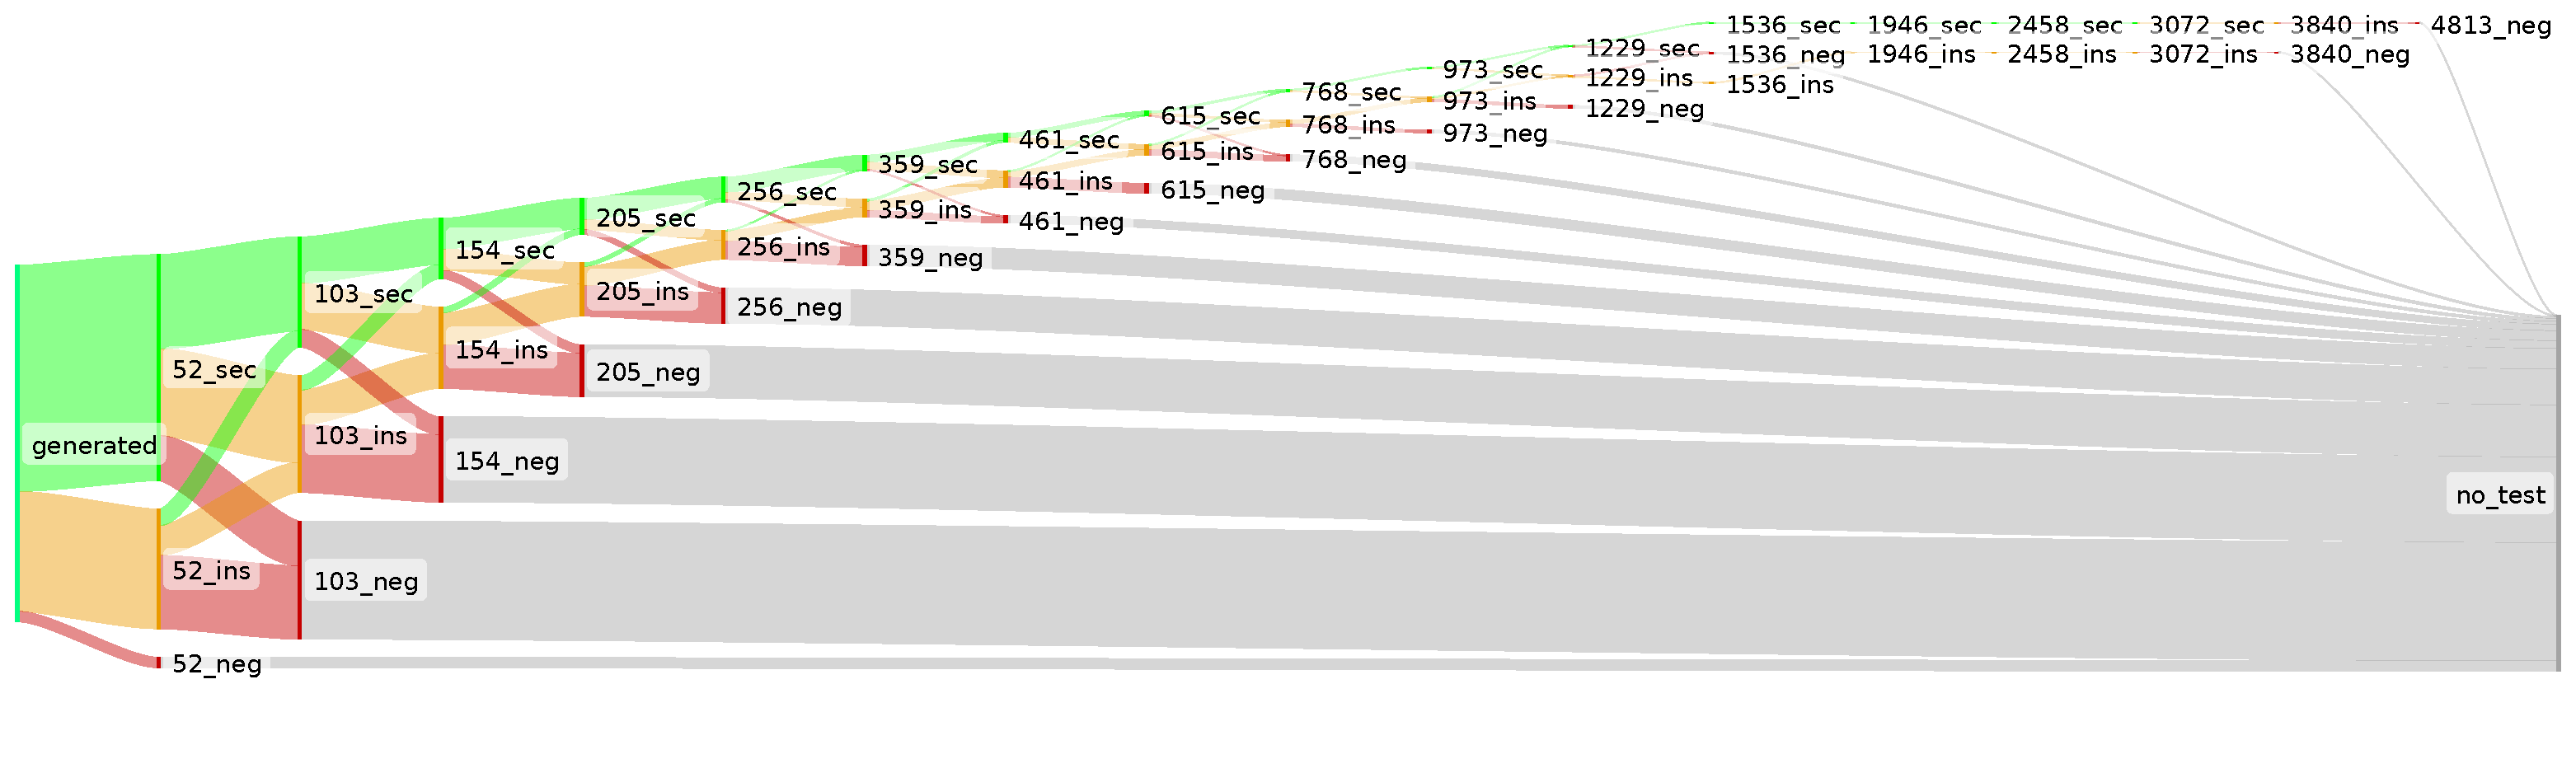
\includegraphics[width=\gsize]{graphs/medium2.old.pdf}
  \caption{Experimental results: performance on random protocols under increasing test power.
    This Sankey plot shows the results of running \toolname on 500 randomly generated \langname files at different test powers.
    Each bucket is labeled as "\texttt{[trainN]\_[result]}", where \texttt{sec} means "appears secure",
    \texttt{ins} means "appears insecure at $\alpha=0.05$",
    and \texttt{neg} means "negligible (insecure at $\alpha=1.25 \cdot 10^{-4}$)".
    Once a program was flagged as negligible, it was not tested at higher test powers.
    For all tests, \texttt{iters=100} and \texttt{testN$\approx\!\!\frac{\mathtt{trainN}}{4}$}.
    }
  \label{fig:sankey}
\end{figure*}

\begin{figure}[tbhp]
  \newcommand{\gsize}{.38\textwidth}
  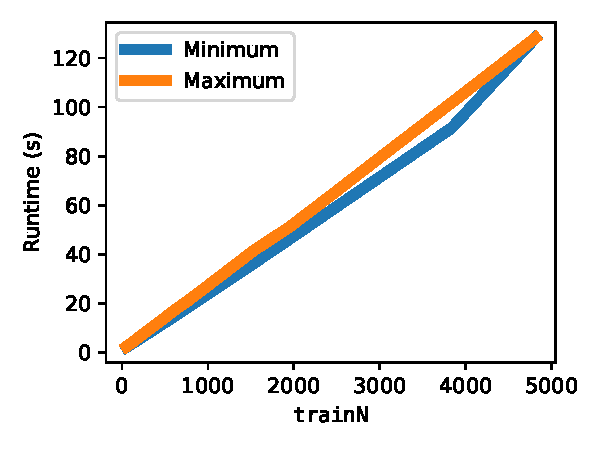
\includegraphics[width=\gsize]{graphs/asymptote_time.pdf} \\
  \caption{Experimental results: runtime with increasing test power. The relation is linear with low variance.
           This data is from the same experiment as Figure~\ref{fig:sankey};
           the number of programs tested diminishes for higher \texttt{trainN} values.
           }
  \label{fig:linear-time}
\end{figure}


\begin{figure*}[tbhp]
  \newcommand{\gsize}{.45\textwidth}
\begin{tabular}{c  c c}
    \rotatebox{90}{\phantom{hellohello}(a). Detection scores (summed)}
  & 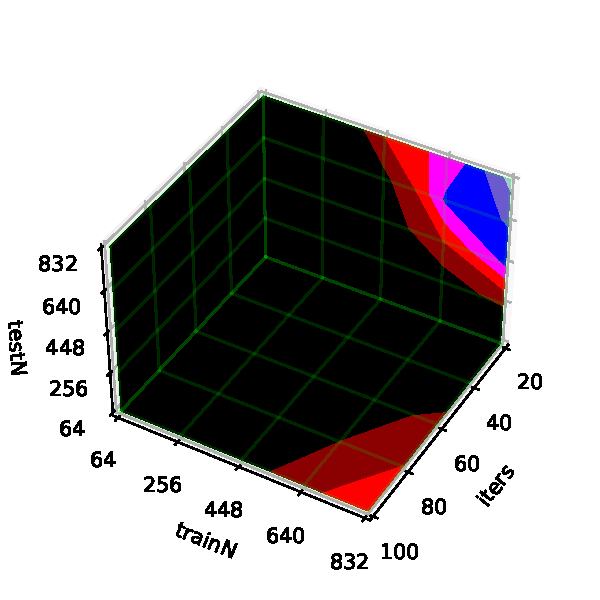
\includegraphics[width=\gsize]{graphs/cube_scores_back.pdf}
  & 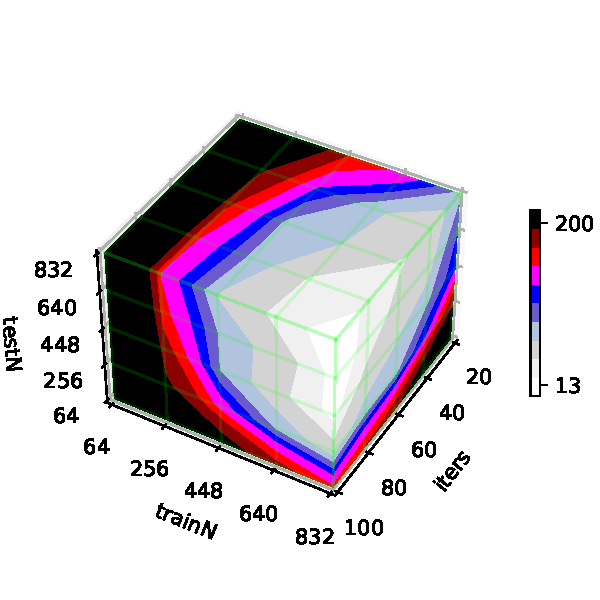
\includegraphics[width=\gsize]{graphs/cube_scores_front.pdf} \\
    \rotatebox{90}{\phantom{hellohellohello}(b). Mean runtime (s)}
  & 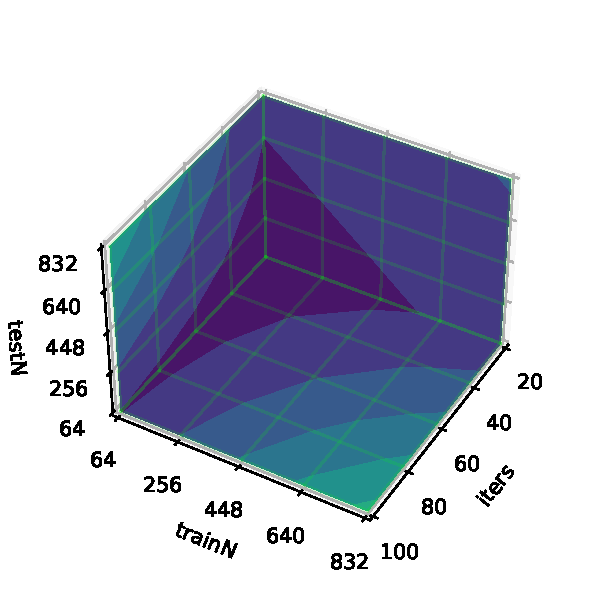
\includegraphics[width=\gsize]{graphs/cube_times_back.pdf}
  & 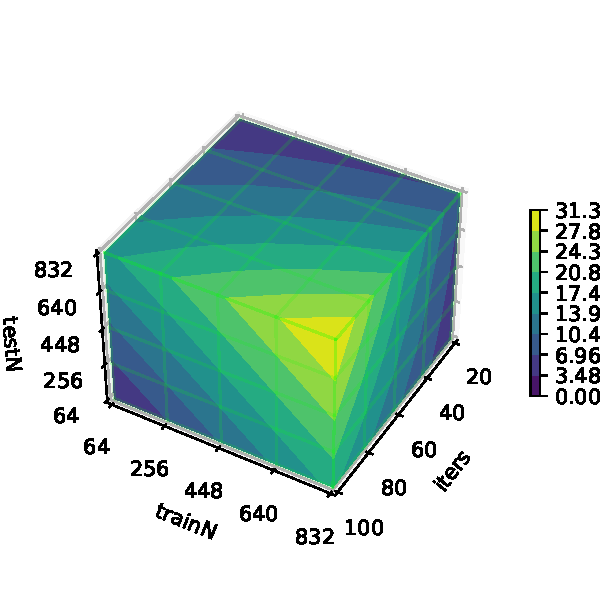
\includegraphics[width=\gsize]{graphs/cube_times_front.pdf} \\
\end{tabular}
\caption{Experimental results: trade-offs in power and runtime under different test parameters.
    $N=200$ at all grid points.
    \textbf{(a)} For each \toolname configuration, we ascribe each protocol a score depending on the test results, and sum the scores.
    Since (per our earlier experiment) statistically all of the protocols are insecure, a lower score indicates better performance by \toolname.
    \textbf{(b)} The mean rumtime of \toolname in this experiment, in seconds.
    The isolines are consistent with the expectation that runtime is driven linearly by the total amount of data used.}
\label{fig:cube-search}
\end{figure*}

\subsection{Results}
Figure~\ref{fig:sankey} shows that, while some programs appear secure at weaker test powers,
all the programs generated with these settings were identified as insecure with $\texttt{iters}=100$ and $\texttt{trainN}<4000$.
Because there's always a chance (at most $\alpha$) of a secure protocol being flagged insecure,
\langname{}s sometimes move back to "secure" from "insecure"; we continue testing them until they reach "negligible".
Figure~\ref{fig:linear-time} shows time data from this same experiment;
because fewer programs were subjected to the larger tests, the minimum and maximum runtimes converge at the end.
More importantly, the runtime scales linearly with the amount of data used in the test.

Figure~\ref{fig:cube-search} shows the individual effects of \texttt{iters}, \texttt{trainN}, and \texttt{testN} on \toolname's power and runtime.
Each 3D heatmap shows aggregate data for 200 randomly generated \toolname files.
Runtime is linear with the amount of data consumed, $\texttt{iters} \cdot (\texttt{trainN} + \texttt{testN})$.
To maximize the granularity of the test-power analysis, we calculate a score for each protocol at each combination of parameters,
where apparently-secure programs count for 2 points,
programs insecure at $\alpha=0.05$ count for 1 point,
and programs insecure at $\alpha=0.01$ count for zero.
Lower scores are "better" because we know virtually all the programs turn out to be actually insecure.
We observe that scaling all three parameters is desirable,
but \texttt{trainN} should generally be larger than \texttt{testN},
and \texttt{iters} may be much smaller.


\section{Evaluation: Bug-Finding in Real-World Protocols}
\label{sec:case-study-protocols}

Our second set of experiments evaluates \toolname's ability to detect security bugs in real-world protocols.
We implement two MPC frameworks for evaluating circuits,
instantiate them with three different functionality-circuits to obtain concrete protocols,
systematically introduce bugs into these protocols,
and evaluate \toolname's ability to detect the bugs.
\toolname is not intended to replace more formal proofs of security,
but rather as a \emph{"sanity check"} before investing effort in such a proof and/or after implementing actual software.
Therefore, the bugs we introduce in these experiments are intended to represent (the statistical effects of) oversights a protocol author might make.
We summarize the implemented protocols in Section~\ref{sec:protocols-evaluated},
describe the experiment and protocol-mutations in Section~\ref{sec:e2-experiment-setup},
and present the results in Section~\ref{sec:e2_results}.

\subsection{Protocols Evaluated}
\label{sec:protocols-evaluated}

For our evaluation, we consider two MPC frameworks for evaluating boolean-arithmetic circuits,
and instantiate those frameworks with three different functions (represented as circuits) to construct secure protocols.
The frameworks and functions are listed in Figure~\ref{fig:protocols} and described below.
All of these protocols are implemented for two parties,
with the addition of a third "dealer" party to produce correlated randomness in the Beaver triple framework.

\begin{figure}
  \centering
  \renewcommand*{\arraystretch}{1.2}
  \begin{tabular}{|l c c l|}
    \hline
      \textbf{MPC Frameworks} & \multicolumn{3}{l |}{\textbf{Approach}} \\
    \hline
    GMW~\cite{goldreich2019play, goldreich2009foundations}
      & \multicolumn{3}{l |}{\begin{minipage}[t]{20em}
      Additively-homomorphic secret sharing, using \textbf{oblivious transfer} for \texttt{AND} gates.\end{minipage}}
    \\ \multicolumn{4}{|c|}{}\\[-1em]
    MPC with Beaver Triples~\cite{beaver1992efficient}
      & \multicolumn{3}{l |}{\begin{minipage}[t]{22em}
          Additively-homomorphic secret sharing, consuming one \textbf{Beaver triple} for each \texttt{AND} gate.\end{minipage}}
    \\ \multicolumn{4}{|c|}{}\\[-1em]
    \hline
    \multicolumn{4}{c}{}\\[-1em]
    \hline
                                      & \textbf{Input} & \textbf{Output} &                       \\[-0.3em]
      \textbf{Instantiated Functions} & \textbf{Width} & \textbf{Width}  & \textbf{Invertibility}\\
    \hline
      $n$-bit Addition             & $n$ & $n$ & Complete \\
      $n$-bit Less-than Comparison & $n$ & $1$ & Partial \\
      Create $n$ Beaver Triples    & $n$ & $n$ & None \\
    \hline
  \end{tabular}
  \bigskip
  \caption{MPC frameworks and instantiated functions used in our evaluation. Each framework describes an approach for evaluating a binary circuit in MPC; we instantiate both frameworks with three different functions (represented as circuits) to construct secure protocols. }
  \label{fig:protocols}
\end{figure}

\paragraph{GMW (Goldreich-Micali-Widgerson).}
The GMW protocol~\cite{goldreich2019play, goldreich2009foundations} is an MPC protocol for evaluating circuits. Each party holds \emph{additive secret shares} of each wire's value; to secret share a bit, a party selects a random bit to represent one share, and computes the other share by XORing the random bit with the secret bit.
%
The parties evaluate addition gates (and other linear operations) by adding the shares they hold.
%
The parties evaluate multiplication gates by using 1-out-of-4 oblivious transfer: the first party generates a random bit for its share of the output, and acts as the sender in OT; the second party acts as the receiver in OT and receives its share of the output. We implemented a compiler to generate \langname programs that evaluate Bristol fashion circuits using GMW.

\paragraph{MPC with Beaver Triples.}
Another MPC protocol for evaluating circuits also uses additive shares to hold wire values,
but uses \emph{Beaver triples}~\cite{beaver1992efficient} to evaluate multiplication gates (instead of OT).
A Beaver triple (or \emph{multiplication triple}) is a set of secret shares of numbers $a$, $b$, and $c$ such that $a \cdot b = c$.
To use a Beaver triple, $P_1$ must have one share of each of $a$, $b$, and $c$, and $P_2$ must have the other share.
Since the values are secret shared, they appear random to each party---but
the correlation between the three numbers can be used to perform efficient multiplication between secret-shared numbers.
To evaluate a multiplication gate with a Beaver triple,
the parties perform two multiplication-by-constant and broadcast operations, and derive one share each of the product.

One Beaver triple must be consumed for each multiplication.
Our implementation of this framework employs a third-party "dealer" who generates the triples on-the-fly;
a pre-processing (offline) phase would be used in real applications.
We implemented a similar compiler to generate \langname programs leveraging this approach for circuit specifications.


\paragraph{Functions evaluated.}
We evaluate three functions, which we express as binary Bristol fashion circuits~\cite{bristol_circuits_website} for two parties
and compile to \langname programs using both of the approaches described above.
All three functions expect input from both the honest and corrupt party.
All three functions are parameterized by their size; their input- and/or output-bit-width is adjustable.
The first, an $n$-bit addition circuit, is vacuously secure;
its ideal functionality leaks all of the honest party's inputs
because the corrupt party can subtract their inputs from the $n$-bit result to reconstruct the honest party's inputs.
The second, an $n$-bit less-than comparison circuit,
only reveals a single bit of information:
which of the two inputs ($n$-bit binary numbers) is larger.
For $n=1$, less-than implementations are also vacuously secure,
but for $n>1$ only partial information about the honest party's inputs is revealed by the ideal functionality.
The third, an $n$-bit Beaver triple generator, leaks no information about the honest party's input,
since its output to each party is a single secret share of the Beaver triple.



\subsection{Experiment Setup}
\label{sec:e2-experiment-setup}

We run \toolname on the unmodified protocol in order to establish the protocol's security
and show that \toolname doesn't flag secure protocols as insecure.
Then we mutate the protocol in several ways to introduce security bugs and test \toolname's ability to detect these bugs.
The effect of each mutation depends on the base protocol to which it's applied;
Figure~\ref{fig:errors} outlines the implications of each mutation to each of the six secure protocols.
Our mutations are:
%
\begin{itemize}
\item \textbf{Biased sharing}: Uses biased randomness to construct secret shares of honest party inputs.
    Specifically, the relevant \inlinecode{FLIP} is replaced by the \inlinecode{AND} of two \inlinecode{FLIP}s.
\item \textbf{Biased AND}: Uses biased randomness (similar to Biased Sharing) as part of the evaluation of multiplication gates.
\item \textbf{Accidental secret}: Sometimes, at random, "accidentally" sends a secret held by the honest party to the corrupt party.
\item \textbf{Accidental gate}: Sometimes, at random, "accidentally" sends an honest party's share of the output wire
    of a multiplication gate to the corrupt party.
\end{itemize}

\begin{figure}
  \centering
  \renewcommand*{\arraystretch}{1.2}
  \begin{tabular}{| r r | c : c : c : c|}
    \hline
      && \textbf{Biased}  & \textbf{Biased}       & \textbf{Accidental} & \textbf{Accidental} \\
      && \textbf{Sharing} & \textbf{AND${}^\ast$} & \textbf{Secret}     & \textbf{Gate} \\
    \hline
      \multirow{3}{*}{\STAB{\rotatebox[origin=lB]{90}{\textbf{\quad GMW\vphantom{p} \quad}}}}
      & \STAB{\rotatebox[origin=lB]{90}{\textbf{\quad Addition\vphantom{p} \quad}}}
      & \multicolumn{4}{c|}{\begin{minipage}[t][][c]{0.6\textwidth}
          % GMW ADDITION ALL CASES
          \cellcolor{nullmutation}
          Because addition is invertible, these are all \emph{vacuously secure}.
        \end{minipage}}
      \\
      \cdashline{2-6}[0.4em/0.5em]
      & \STAB{\rotatebox[origin=lB]{90}{\textbf{\quad Less Than${}^\dagger$\vphantom{p} \quad}}}
      & \begin{minipage}[c][][c]{0.204\textwidth}
          %GMW LESS THAN BIASED SHARING
          \cellcolor{insecmutation}
          Insecure
        \end{minipage}
      & \begin{minipage}[c][][c]{0.204\textwidth}
          %GMW LESS THAN BIASED AND
          \cellcolor{insecmutation}
          Insecure
        \end{minipage}
      & \begin{minipage}[c][][c]{0.204\textwidth}
          %GMW LESS THAN ACCIDENTIAL SECRET
          \cellcolor{insecmutation}
          Insecure
        \end{minipage}
      & \begin{minipage}[c][][c]{0.204\textwidth}
          %GMW LESS THAN ACCIDENTIAL GATE
          \cellcolor{insecmutation}
          Insecure
        \end{minipage}
      \\
      \cdashline{2-6}[0.4em/0.5em]
      & \STAB{\rotatebox[origin=lB]{90}{\textbf{\quad Make Beaver Triples \quad}}}
      & \begin{minipage}[c][][c]{0.204\textwidth}
          % GMW MAKE BEAVER TRIPLES BIASED SHARING
          \cellcolor{insecmutation}
          Insecure
        \end{minipage}
      & \begin{minipage}[c][][c]{0.204\textwidth}
          %GMW MAKE BEAVER TRIPLES BIASED AND
          \cellcolor{nullmutation}
          Secure.
          Since the \texttt{AND} gates are exactly the output-wires of the circuits, leaking them doesn't reveal anything additional.
        \end{minipage}
      & \begin{minipage}[c][][c]{0.204\textwidth}
          %GMW MAKE BEAVER TRIPLES ACCIDENTIAL SECRET
          \cellcolor{insecmutation}
          Insecure
        \end{minipage}
      & \begin{minipage}[c][][c]{0.204\textwidth}
          %GMW MAKE BEAVER TRIPLES ACCIDENTIAL GATE
          \cellcolor{nullmutation}
          Secure.
          Since the \texttt{AND} gates are exactly the output-wires of the circuits, leaking them doesn't reveal anything additional.
        \end{minipage}
      \\
      \hdashline[0.5em/0.4em]
      \multirow{3}{*}{\STAB{\rotatebox[origin=lB]{90}{\textbf{\quad MPC with Beaver Triples \quad}}}}
      & \STAB{\rotatebox[origin=lB]{90}{\textbf{\quad Addition\vphantom{p} \quad}}}
      & \multicolumn{4}{c|}{\begin{minipage}[t][][c]{0.6\textwidth}
          % BEAVER ADDITION BANNER
          \cellcolor{nullmutation}
          Because addition is invertible, these are all \emph{vacuously secure}.
        \end{minipage}}
      \\
      \cdashline{2-6}[0.4em/0.5em]
      & \STAB{\rotatebox[origin=lB]{90}{\textbf{\quad Less Than${}^\dagger$\vphantom{p} \quad}}}
      & \begin{minipage}[t][][c]{0.204\textwidth}
          % BEAVER LESS THAN BIASED SHARING
          \cellcolor{insecmutation}
          Insecure
        \end{minipage}
      & \begin{minipage}[c][][c]{0.204\textwidth}
          %BEAVER LESS THAN BIASED AND
          \cellcolor{insecmutation}
          \vspace*{4pt}
          Insecure.
          The biased \inlinecode{FLIP}s happen within the dealer party;
          the inverse-computation needed to leverage them is much deeper for this version of the mutation.\vspace*{4pt}
        \end{minipage}
      & \begin{minipage}[c][][c]{0.204\textwidth}
          %BEAVER LESS THAN ACCIDENTIAL SECRET
          \cellcolor{insecmutation}
          Insecure
        \end{minipage}
      & \begin{minipage}[c][][c]{0.204\textwidth}
          %BEAVER LESS THAN ACCIDENTIAL GATE
          \cellcolor{insecmutation}
          Insecure
        \end{minipage}
      \\
      \cdashline{2-6}[0.4em/0.5em]
      & \STAB{\rotatebox[origin=lB]{90}{\textbf{\quad Make Beaver Triples \quad}}}
      & \begin{minipage}[c][][c]{0.204\textwidth}
          %BEAVER MAKE BEAVER TRIPLES BIASED SHARING
          \cellcolor{insecmutation}
          Insecure
        \end{minipage}
      & \begin{minipage}[c][][c]{0.204\textwidth}
          %BEAVER MAKE BEAVER TRIPLES BIASED AND
          \cellcolor{insecmutation}
          Insecure.
          \inlinecode{C} has a good guess of the true shared triple.
        \end{minipage}
      & \begin{minipage}[c][][c]{0.204\textwidth}
          %BEAVER MAKE BEAVER TRIPLES ACCIDENTIAL SECRET
          \cellcolor{insecmutation}
          Insecure
        \end{minipage}
      & \begin{minipage}[c][][c]{0.204\textwidth}
          %BEAVER MAKE BEAVER TRIPLES ACCIDENTIAL GATE
          \cellcolor{nullmutation}
          Secure.
          Since the \texttt{AND} gates are exactly the output-wires of the circuits, leaking them doesn't reveal anything additional.
        \end{minipage}
      \\
    \hline
  \end{tabular}
  \caption{Expected results.
  In eleven of the twenty four mutation cases (\highlight{nullmutation}{in gray}) the protocol will remain secure.\\
  \footnotesize{$\ast$ \textbf{Biased AND} is implemented differently in the two frameworks.}\\
  \footnotesize{$\dagger$ For $n=1$, the \textbf{Less Than} protocols are all \emph{vacuously secure}.}}
  \label{fig:errors}
\end{figure}


\subsection{Results}
\label{sec:e2_results}

Each of the thirty combinations of framework, functionality, and mutation (including un-mutated)
was instantiated with different values of $n$ from $1-32$ and tested with \toolname at four different power-settings in the low-to-medium range.
(Each combination of \langname-file and \toolname-configuration was run three times to account for stochastic behavior.)
Other than the $n=1$ cases, these variations within each combination mostly did not affect the outcomes of the tests.
(They did affect runtime of the tests, which scaled linearly with the quantity of view-data generated/consumed.)
In Figure~\ref{fig:observations} we summarize these outcomes.
Figure~\ref{fig:observations-detail} shows detailed $p$-value and runtime data for the case of Beaver triple generation using the GMW framework.
More complete experimental results appear in Appendix~\ref{sec:addit-exper-results}.

\begin{figure}
  \centering
  \renewcommand*{\arraystretch}{1.2}
  \begin{tabular}{| r r | c : c : c : c|}
    \hline
      && \textbf{Biased} &  \textbf{Biased} & \textbf{Accidental} & \textbf{Accidental} \\
      && \textbf{Sharing} & \textbf{AND} &    \textbf{Secret} &     \textbf{Gate} \\
    \hline
      \multirow{3}{*}{\STAB{\rotatebox[origin=lB]{90}{\textbf{\quad GMW\vphantom{p} \quad}}}}
      & \STAB{\rotatebox[origin=lB]{90}{\textbf{\quad Addition\vphantom{p} \quad}}}
      & \begin{minipage}[t][][c]{0.204\textwidth}
          %GMW ADDITION BIASED SHARING
          \cellcolor{incorrect}
          \texttt{INSECURE}
          (for $n>10$)${}^\ddagger$
        \end{minipage}
      & \begin{minipage}[t][][c]{0.204\textwidth}
          %GMW ADDITION BIASED AND
          \cellcolor{incorrect}
          \texttt{INSECURE}
          (for $n>7$)${}^\ddagger$
        \end{minipage}
      & \begin{minipage}[t][][c]{0.204\textwidth}
          %GMW ADDITION ACCIDENTIAL SECRET
          \cellcolor{incorrect}
          \texttt{INSECURE}
          (for $n>10$)${}^\ddagger$
        \end{minipage}
      & \begin{minipage}[t][][c]{0.204\textwidth}
          %GMW ADDITION ACCIDENTIAL GATE
          \cellcolor{correct}
          \texttt{MAYBE SECURE}
        \end{minipage}
      \\
      \cdashline{2-6}[0.4em/0.5em]
      & \STAB{\rotatebox[origin=lB]{90}{\textbf{\quad Less Than${}^\dagger$\vphantom{p} \quad}}}
      & \begin{minipage}[t][][c]{0.204\textwidth}
          %GMW LESS THAN BIASED SHARING
          \cellcolor{correct}
          \texttt{INSECURE}
        \end{minipage}
      & \begin{minipage}[t][][c]{0.204\textwidth}
          %GMW LESS THAN BIASED AND
          \cellcolor{correct}
          \texttt{INSECURE}
        \end{minipage}
      & \begin{minipage}[t][][c]{0.204\textwidth}
          %GMW LESS THAN ACCIDENTIAL SECRET
          \cellcolor{correct}
          \texttt{INSECURE}
        \end{minipage}
      & \begin{minipage}[t][][c]{0.204\textwidth}
          %GMW LESS THAN ACCIDENTIAL GATE
          \cellcolor{correct}
          \texttt{INSECURE}
        \end{minipage}
      \\
      \cdashline{2-6}[0.4em/0.5em]
      & \STAB{\rotatebox[origin=lB]{90}{\textbf{\quad Make Beaver Triples \quad}}}
      & \begin{minipage}[t][][c]{0.204\textwidth}
          %GMW MAKE BEAVER TRIPLES BIASED SHARING
          \cellcolor{correct}
          \texttt{INSECURE}
        \end{minipage}
      & \begin{minipage}[t][][c]{0.204\textwidth}
          %GMW MAKE BEAVER TRIPLES BIASED AND
          \cellcolor{correct}
          \texttt{MAYBE SECURE}
        \end{minipage}
      & \begin{minipage}[t][][c]{0.204\textwidth}
          %GMW MAKE BEAVER TRIPLES ACCIDENTIAL SECRET
          \cellcolor{correct}
          \texttt{INSECURE}
        \end{minipage}
      & \begin{minipage}[t][][c]{0.204\textwidth}
          %GMW MAKE BEAVER TRIPLES ACCIDENTIAL GATE
          \cellcolor{correct}
          \texttt{MAYBE SECURE}
        \end{minipage}
      \\
      \hdashline[0.5em/0.4em]
      \multirow{3}{*}{\STAB{\rotatebox[origin=lB]{90}{\textbf{\quad MPC with Beaver Triples \quad}}}}
      & \STAB{\rotatebox[origin=lB]{90}{\textbf{\quad Addition\vphantom{p} \quad}}}
      & \begin{minipage}[t][][c]{0.204\textwidth}
          %BEAVER ADDITION BIASED SHARING
          \cellcolor{incorrect}
          \texttt{INSECURE}
          (for $n>10$)${}^\ddagger$
        \end{minipage}
      & \begin{minipage}[t][][c]{0.204\textwidth}
          %BEAVER ADDITION BIASED AND
          \cellcolor{correct}
          \texttt{MAYBE SECURE}
        \end{minipage}
      & \begin{minipage}[t][][c]{0.204\textwidth}
          %BEAVER ADDITION ACCIDENTIAL SECRET
          \cellcolor{incorrect}
          \texttt{INSECURE}
          (for $n>7$)${}^\ddagger$
        \end{minipage}
      & \begin{minipage}[t][][c]{0.204\textwidth}
          %BEAVER ADDITION ACCIDENTIAL GATE
          \cellcolor{correct}
          \texttt{MAYBE SECURE}
        \end{minipage}
      \\
      \cdashline{2-6}[0.4em/0.5em]
      & \STAB{\rotatebox[origin=lB]{90}{\textbf{\quad Less Than${}^\dagger$\vphantom{p} \quad}}}
      & \begin{minipage}[t][][c]{0.204\textwidth}
          %BEAVER LESS THAN BIASED SHARING
          \cellcolor{correct}
          \texttt{INSECURE}
        \end{minipage}
      & \begin{minipage}[t][][c]{0.204\textwidth}
          %BEAVER LESS THAN BIASED AND
          \cellcolor{incorrect}
          \texttt{MAYBE SECURE}
        \end{minipage}
      & \begin{minipage}[t][][c]{0.204\textwidth}
          %BEAVER LESS THAN ACCIDENTIAL SECRET
          \cellcolor{correct}
          \texttt{INSECURE}
        \end{minipage}
      & \begin{minipage}[t][][c]{0.204\textwidth}
          %BEAVER LESS THAN ACCIDENTIAL GATE
          \cellcolor{incorrect}
          \texttt{MAYBE SECURE}
        \end{minipage}
      \\
      \cdashline{2-6}[0.4em/0.5em]
      & \STAB{\rotatebox[origin=lB]{90}{\textbf{\quad Make Beaver Triples \quad}}}
      & \begin{minipage}[t][][c]{0.204\textwidth}
          %BEAVER MAKE BEAVER TRIPLES BIASED SHARING
          \cellcolor{correct}
          \texttt{INSECURE}
        \end{minipage}
      & \begin{minipage}[t][][c]{0.204\textwidth}
          %BEAVER MAKE BEAVER TRIPLES BIASED AND
          \cellcolor{correct}
          \texttt{INSECURE}
        \end{minipage}
      & \begin{minipage}[t][][c]{0.204\textwidth}
          %BEAVER MAKE BEAVER TRIPLES ACCIDENTIAL SECRET
          \cellcolor{correct}
          \texttt{INSECURE}
        \end{minipage}
      & \begin{minipage}[t][][c]{0.204\textwidth}
          %BEAVER MAKE BEAVER TRIPLES ACCIDENTIAL GATE
          \cellcolor{correct}
          \texttt{MAYBE SECURE}
        \end{minipage}
      \\
    \hline
  \end{tabular}
  \bigskip
  \caption{Observed results.
  Seventeen of the twenty four mutation cases are correctly flagged by \toolname (\highlight{correct}{in green});
  in other cases (\highlight{incorrect}{in red}) an insecure protocol is not detected, or a vacuously secure protocol is flagged as \texttt{INSECURE}.\\
  \footnotesize{$\dagger$ Since \textbf{Less Than} protocols are \emph{vacuously secure} at $n=1$, those cases are not represented here.}\\
  \footnotesize{$\ddagger$ See Figure~\ref{fig:interpretation}a2.}}
  \label{fig:observations}
\end{figure}

\begin{figure*}
  \centering
  \newcommand{\gsize}{.45\textwidth}
\begin{tabular}{c c}
    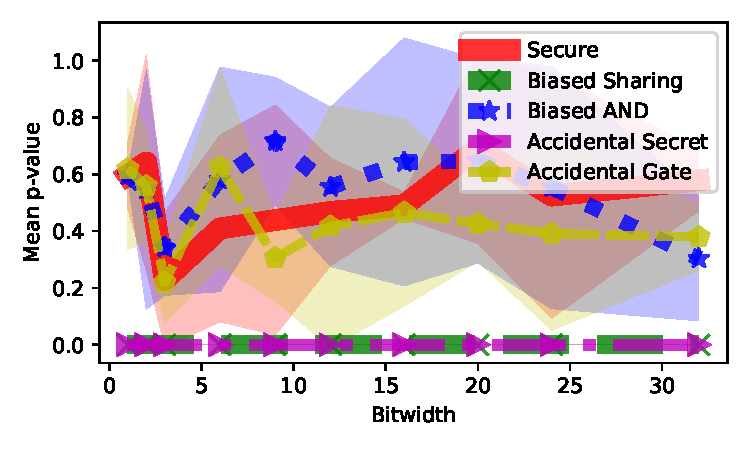
\includegraphics[width=\gsize]{graphs/security_beaver_triple_gen_gmw_128_1024.pdf} &
    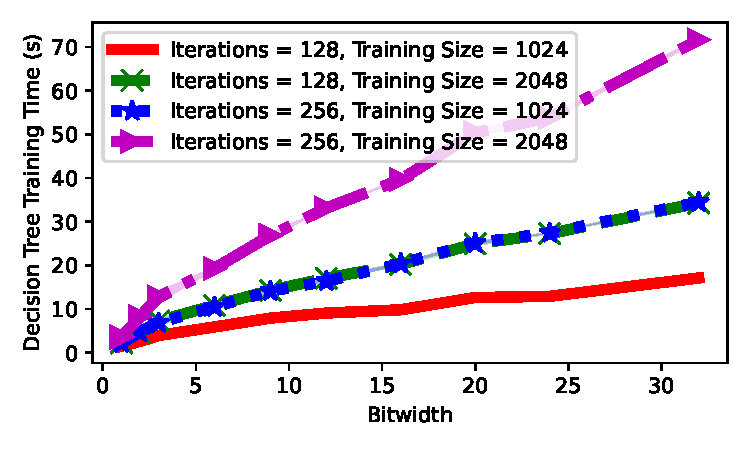
\includegraphics[width=\gsize]{graphs/time_beaver_triple_gen_gmw_256_2048.pdf} \\
    \textit{(a.)} & \textit{(b.)}
\end{tabular}
\caption{Experimental results from running \toolname against GMW implementations of Beaver triple generation.
    \textit{(a.)} Keeping \texttt{iters=128}, \texttt{trainN=1024}, and \todo{testN=?}, we report the average of the returned $p$-values
      for different mutation-settings and bit-widths, with error-bars as background shading;
      $N=3$ for each data-point, so there is still some noise.
    \textit{(b.)} We report the average runtime of \toolname with different power-settings against protocols of different bit-widths.
      We report only the time taken by the \toolname test, not the time taken to \emph{generate} the data provided to it.
      \todo{These are all the secure version, right?}}
\label{fig:observations-detail}
\end{figure*}


\paragraph{Detecting security bugs.}
\toolname is able to detect most, but not all, security bugs in our evaluation.
Of the thirteen actually-insecure protocols (we ignore bit-width for the moment), eleven reliably received \texttt{INSECURE}.
In these cases, the $p$-values were consistently negligible.
In the Beaver triple based framework, some errors were not detected that ideally would have been.
Due to the use of multiplication triples, taking advantage of the leakage from incorrectly-implemented \texttt{AND} gates
in this framework is much more difficult than in the GMW case.
These results suggest that \toolname will likely have difficulty detecting bugs that require deep ``backwards computation''
to leverage the leaked information.

In Figure~\ref{fig:interpretation} we noted a possible situation in which a secure protocol might be flagged \texttt{INSECURE},
not by chance, but because information nominally inferable in the ideal world was not inferred by the ideal-world-trained D-Trees
due to insufficient training data
(and was inferred or better-inferred by the real-world trained D-Trees).
As expected, this was only a problem with the vacuously secure Addition protocols
that had been mutated in ways that \emph{"should have"} made them insecure.
Vacuously secure protocols are of little interest in terms of MPC applications,
and it's unclear if this kind of false-\texttt{INSECURE} report could happen
to a real protocol that was correct to its authors intentions.

For protocols reported as \texttt{INSECURE}, the $p$-values were usually negligible.
Intermediate behavior, where the $p$-values are biased-low but not consistently below reasonable $\alpha$ thresholds,
requires improbable alignment of the difficulty of detecting the bug and the power-configuration of \toolname.
For protocols reported as \texttt{MAYBE SECURE}, the $p$-values tend to be \emph{either} uniformly distributed
\emph{or} consistently approximately-equal-to one.


\paragraph{Scalability.}
The primary computational cost of \toolname is the time taken to train the decision trees.
For the settings we evaluated, training time grows linearly with the number of iterations,
the training data size, and the bitwidth of the target function (\ie the size of the circuit being tested).
Even for the largest bitwidths and row-counts we considered, training takes only minutes.


\subsection{Discussion}

The results of these experiments suggest that \toolname scales linearly with protocol size and test power,
and is capable of detecting bugs in both randomly-generated and real-world protocols.
The test typically runs in just seconds to minutes.
The results of our experiment on protocol mutations show that \toolname is effective for detecting important classes of security bugs,
but that care must be taken in interpreting the results.

For security bugs that directly reveal sensitive information (\eg \textbf{biased sharing} bugs) \toolname is particularly effective.
Our results suggest that \toolname is capable of detecting these accidental disclosures even at low test powers and in the context of large protocols.

\toolname is less effective for security bugs that require significant ``backwards computation'' to leverage the leaked information
(\eg \textbf{accidental gate} bugs), since decision trees are not well-suited to solving this problem.
We leave open the possibility that more sophisticated models---such as a deep neural networks---might
be able to perform this kind of inference, but they would take significantly longer to train.



\section{Related Work}

\subsection{Formal-methods for cryptography}
Although automated language-based verification of MPC security is an open question,
a variety of useful work approaches the subject from different directions.

Haagh et al.~\cite{haagh2018computer} % Computer-aided proofs for multiparty computation with active security
use EasyCrypt to manually show the security of GMW.
Their definitions generalize to protocols with efficiently invertible functionalities.
They model MPC as a non-interference property: Honest secrets are non-interfering on the corrupt views conditioned on the corrupt outputs.
Their approach requires manual proof in EasyCrypt.

Barthe et al.~\cite{barthe2019probabilistic} % https://arxiv.org/abs/1907.10708 A Probabilistic Separation Logic
give a framework for probabilistic reasoning and show that it can be used to prove security of additive secret sharing.
However, the framework is not amenable to automation.

Gancher et al.~\cite{gancher2023core} % https://dl.acm.org/doi/pdf/10.1145/3571223
give a powerful language system that can check if one protocol is a valid simulator of another,
and show that it works on existing MPC protocols like GMW.
The user of the system needs to write a second protocol
representing the composition of the ideal-world functionality and an explicit $\mathtt{SIM}$,
and then build a high-level proof of the equivalence in the provided equational logic.

The \textsc{Wysteria} language~\cite{rastogi2014wysteria} % https://www.ieee-security.org/TC/SP2014/papers/Wysteria_c_AProgrammingLanguageforGeneric,Mixed-ModeMultipartyComputations.pdf
gives fine-grained integration of MPC as a language primitive, to help a larger program use it efficiently.
Their system assumes (at least one) secure implementation of MPC on circuits.

$\lambda_\textbf{obliv}$~\cite{darais2019language} %
gives a type system that ensures uniform and independent randomness of key values throughout a program.
Their system is automated, and could be adapted to ensure perfect noninterference between honest secrets and corrupt views,
but does not support the kind of \emph{conditional} independence required for most MPC protocols.

\textsc{Owl}~\cite{gancher2023owl} % https://eprint.iacr.org/2023/473.pdf
gives a type system guaranteeing non-interference with an (extensible) selection of cryptographic operations as language primitives.
OWL is designed for secure protocols that reveal nothing to the adversary, and does not support verification of MPC security.

Fournet et al.~\cite{fournet2011information} % https://www.microsoft.com/en-us/research/wp-content/uploads/2017/01/information-flow-types-for-homomorphic-encryptions-ccs11.pdf
also use a type system to ensure safe usage of cryptographic primitives,
but they specifically work with homomorphic encryption schemes and the various measures by which such schemes may be correct.
Like \textsc{Owl}, their type system assumes a secure implementation of the encryption scheme and does not support verification of MPC security.

\subsection{PPLs for Inference}

Several PPLs directly support efficient inference and some forms of independence testing.
A Sum Product Network (SPN)~\cite{poon2011sum} is a directed-graph representation of a multi-variate distribution;
SPPL~\cite{saad2021sppl} is a PPL that performs inference using SPNs.
SPNs are compact, allow efficient inference, and can represent values symbolically as needed,
so testing for conditional independence is practical.
However, such a language cannot express any existing MPC protocols, and likely cannot express any \emph{useful} protocols,
because if the language allowed any value to be used more than once, it would result in graphs that violate key invariants of SPNs.

The \textsc{Dice} language~\cite{holtzen2020scaling} analogously translates programs into binary decision diagrams (BDDs).
BDDs can represent, and do inference on, distributions that aren't representable as SPNs,
but since the graph \emph{structure} of the BDD of a \textsc{Dice} program depends on the actual \emph{values} on which one is conditioning,
a \textsc{Dice}-based test for the kind of conditional independence needed for MPC would scale exponentially with the input/output width of the protocol.

\textsc{Lilac}~\cite{li2023lilac} % https://arxiv.org/abs/2304.01339
is a program logic for reasoning about probability distributions and PPLs.
It more expressive than the original probabilistic separation logic,
but does not support automation.


\subsection{Probabilistic testing}

Ding et al.~\cite{ding2018detecting} % https://arxiv.org/pdf/1805.10277.pdf
and more recently Zhang et al.~\cite{zhang2020testing} % https://dl.acm.org/doi/10.1145/3428233
use large samples of program executions to test for violations of differential privacy,
showing that such techniques can work on probabilistic hyper-properties.
Since differential privacy is only concerned with program inputs and outputs,
the dimensionality of the problem is somewhat smaller than MPC.

Our work builds directly on that of Chalupka et al.~\cite{chalupka2018fast}
who show that batches of ML classifiers can be used to check conditional independence.
Specifically, if decision trees (D-Trees) trained on random variables $A$ and $C$
do better at predicting the value of a random variable $B$ than D-Trees trained only on $C$,
then $A$ and $B$ are not independent conditioned on $C$.
The test is statistical; many D-Trees are trained and any apparent advantage of the better-informed ones must be assessed for statistical significance.
In their work the data is assumed to be permuted sub-samples of some finite pool of samples from a population,
but in our adaptation we use fresh program traces for everything.

\section{Future Work}

Some further work is needed to turn \toolname into a deploy-able tool;
our experiments so far are not sufficient to calculate sensible default settings,
and we believe some changes to the way the data is ingested and handled by the tool could improve efficiency.

There are also variations on the core concept of \toolname that we believe are worth exploring.
Decision trees are not the only candidate for the underlying ML model, and our evaluation suggests that they are incapable of performing some of the ``backwards computation'' needed to demonstrate insecurity;
a deeper model (\eg a neural network) may be more capable of detecting these kinds of security bugs.
Other cryptographic properties besides MPC can likely be framed in terms of conditional independence;
and so would be amenable to similar tests.
Finally, because end-to-end static analysis of MPC protocols has proven so difficult,
we believe it may be practical to augment a stochastic tool like \toolname with static analysis capabilities
that would allow it to more efficiently detect insecurity, turning it into a "white-box" test.


\section{Conclusions}

We present \toolname,
a property-based test that checks (a small over-approximation of) MPC security
using a probabilistic test of conditional independence.
At its heart, \toolname trains batches of decision trees with and without access to grey-box data from many evaluations of the target protocol
to see if access to that message data improves their ability to predict the secret inputs.
While this approach has theoretical limitations, we show that in practice it is able to detect various mistakes in various protocols,
making it a useful tool for sanity-checking one's work during development.
We also show that, in practice, the compute-time required for \toolname scales linearly with the power of the test requested,
and usefully-powerful tests take just a few minutes.

%%
%% The acknowledgments section is defined using the "acks" environment
%% (and NOT an unnumbered section). This ensures the proper
%% identification of the section in the article metadata, and the
%% consistent spelling of the heading.
\begin{acks}
    \todo{Redacted for submission}
\end{acks}

%%
%% The next two lines define the bibliography style to be used, and
%% the bibliography file.
\bibliographystyle{ACM-Reference-Format}
\bibliography{refs}


%%
%% If your work has an appendix, this is the place to put it.
\appendix

\section{Additional Experimental Results}
\label{sec:addit-exper-results}

This Appendix contains additional experimental results excluded from the main body of the paper:
The results appear in Figures~\ref{fig:results_security} and~\ref{fig:results_training_time}. For the results in Figure~\ref{fig:results_security}, we set the number of iterations to 128 and the training set size to 1024. The results are similar for other settings; additional experimental results appear in Appendix~\ref{sec:addit-exper-results}.
We record the total training time for each combination of MPC framework and function, and plot the results for several settings in Figure~\ref{fig:results_training_time}. 
%
\begin{itemize}
\item Figure~\ref{fig:extra1} presents additional results for $n$-bit addition.
\item Figure~\ref{fig:extra2} presents additional results for $n$-bit less-than comparison.
\item Figure~\ref{fig:extra3} presents additional results for $n$-bit Beaver triple generation.
\end{itemize}


\begin{figure*}
  \centering
  \newcommand{\gsize}{.45\textwidth}
\begin{tabular}{c| c c}
    \hline\hline
  & \textbf{OT-Based (GMW)} & \textbf{Beaver Triple-Based}\\
    \hline\hline
  \rotatebox{90}{\phantom{hellohello}$n$-bit addition}
  & 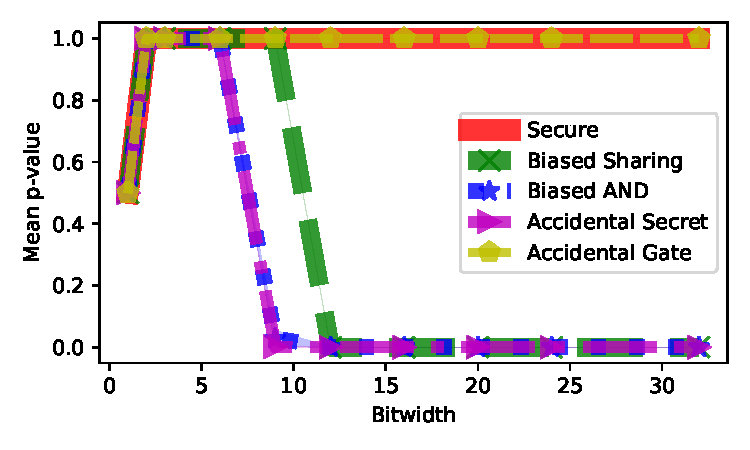
\includegraphics[width=\gsize]{graphs/security_adder_gmw_128_1024.pdf}
                 & 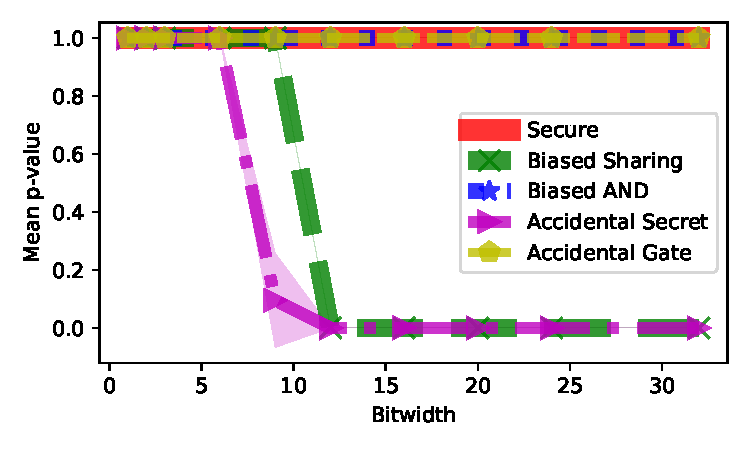
\includegraphics[width=\gsize]{graphs/security_adder_beaver_128_1024.pdf} \\
    \hline
  \rotatebox{90}{\phantom{hel}$n$-bit less-than comparison}
  & 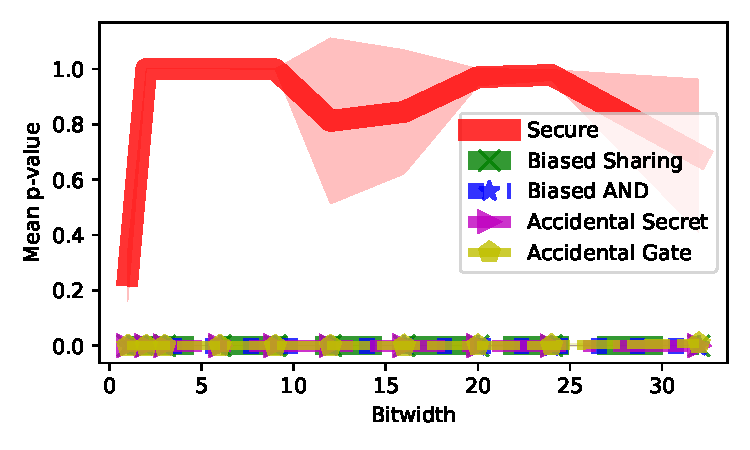
\includegraphics[width=\gsize]{graphs/security_less_than_gmw_128_1024.pdf}
                 & 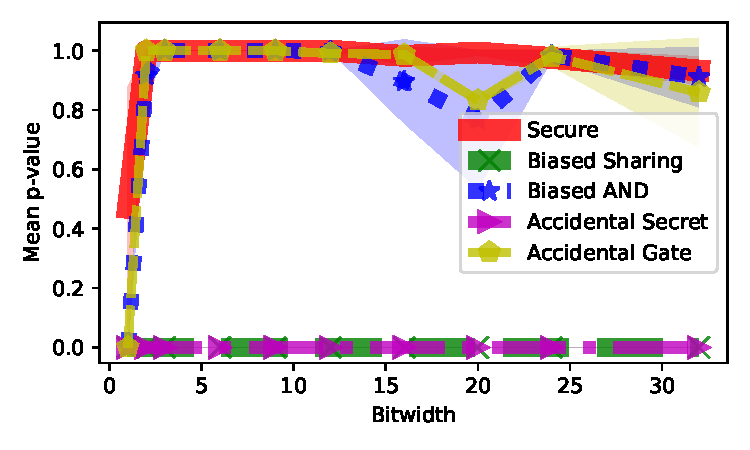
\includegraphics[width=\gsize]{graphs/security_less_than_beaver_128_1024.pdf} \\
    \hline
  \rotatebox{90}{\phantom{h}$n$-bit Beaver triple generation}
  & 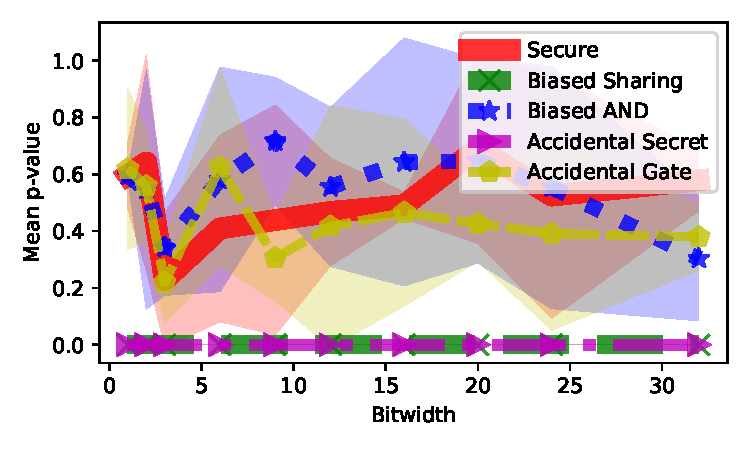
\includegraphics[width=\gsize]{graphs/security_beaver_triple_gen_gmw_128_1024.pdf}
                 & 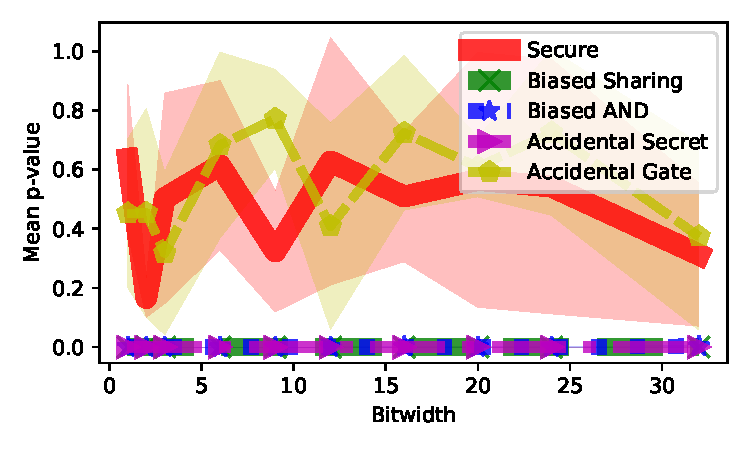
\includegraphics[width=\gsize]{graphs/security_beaver_triple_gen_beaver_128_1024.pdf} \\
    \hline
    \hline
\end{tabular}
\caption{Experimental results: ability to detect security bugs. We set the number of iterations to 128 and the training set size to 1024. Results for other settings appear in Appendix~\ref{sec:addit-exper-results}.}
\label{fig:results_security}
\end{figure*}



\begin{figure*}
  \centering
  \newcommand{\gsize}{.45\textwidth}
\begin{tabular}{c| c c}
    \hline\hline
  & \textbf{OT-Based (GMW)} & \textbf{Beaver Triple-Based}\\
    \hline\hline
  \rotatebox{90}{\phantom{hellohello}$n$-bit addition}
  & 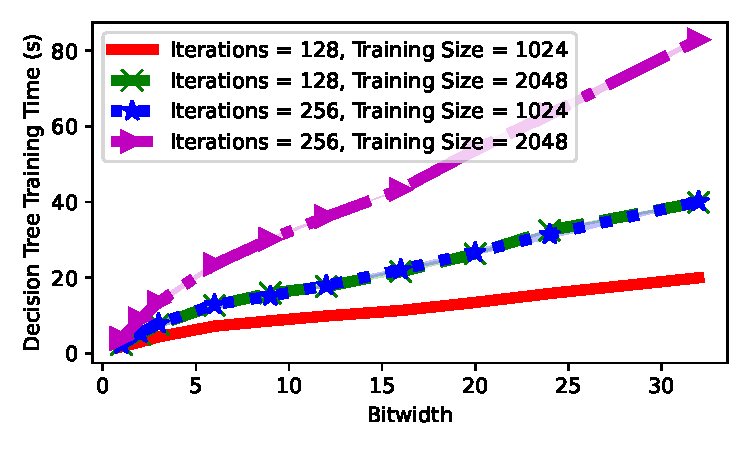
\includegraphics[width=\gsize]{graphs/time_adder_gmw_256_2048.pdf}
                 & 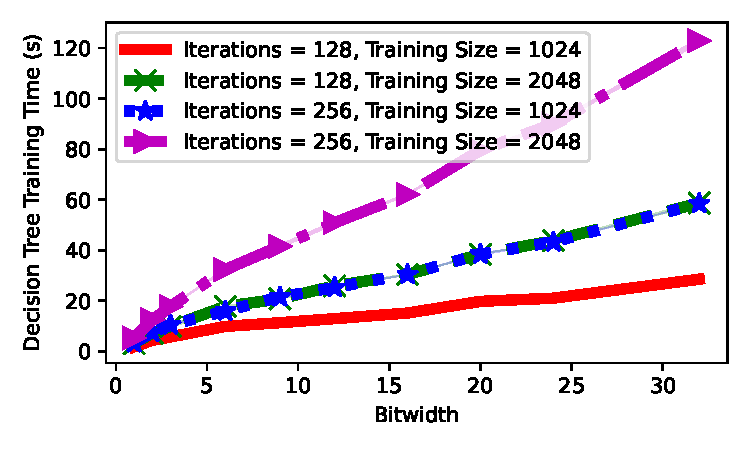
\includegraphics[width=\gsize]{graphs/time_adder_beaver_256_2048.pdf} \\
    \hline
  \rotatebox{90}{\phantom{hel}$n$-bit less-than comparison}
  & 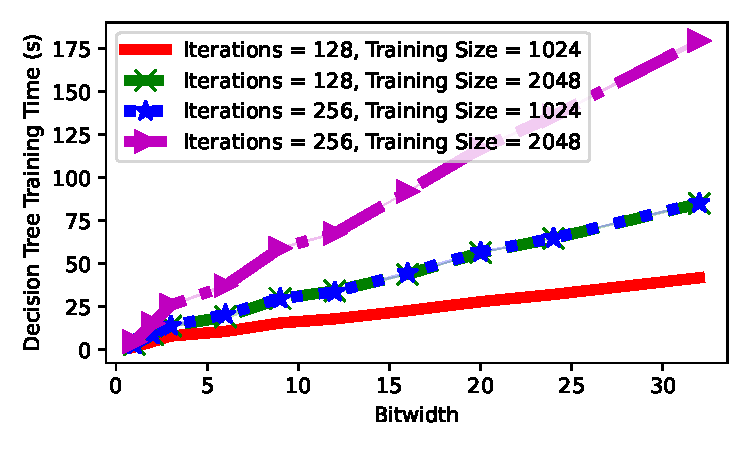
\includegraphics[width=\gsize]{graphs/time_less_than_gmw_256_2048.pdf}
                 & 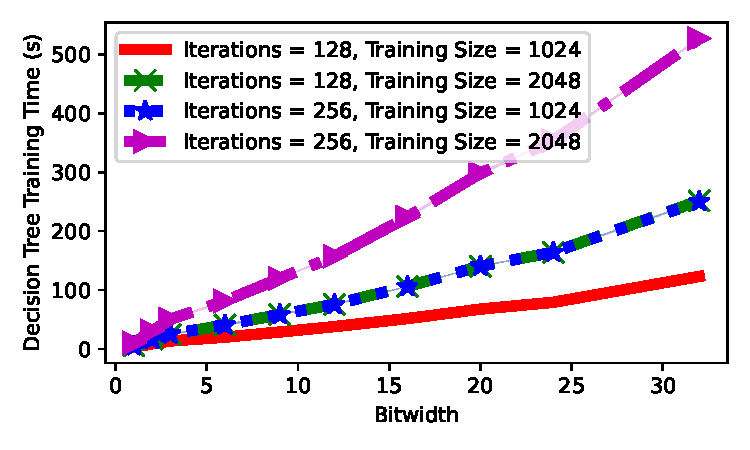
\includegraphics[width=\gsize]{graphs/time_less_than_beaver_256_2048.pdf} \\
    \hline
  \rotatebox{90}{\phantom{h}$n$-bit Beaver triple generation}
  & 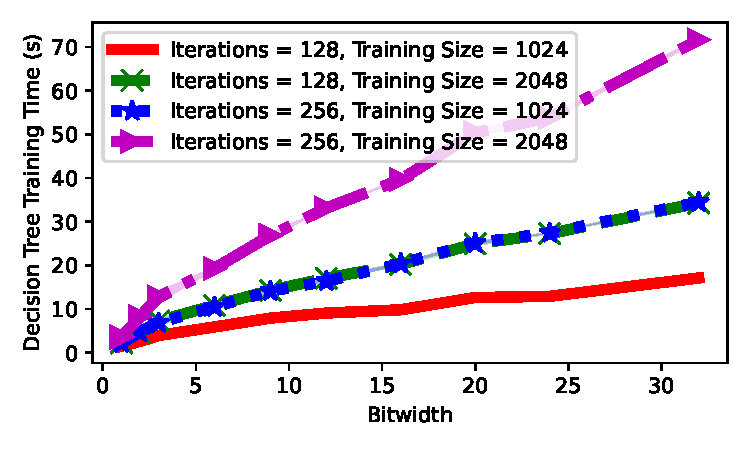
\includegraphics[width=\gsize]{graphs/time_beaver_triple_gen_gmw_256_2048.pdf}
                 & 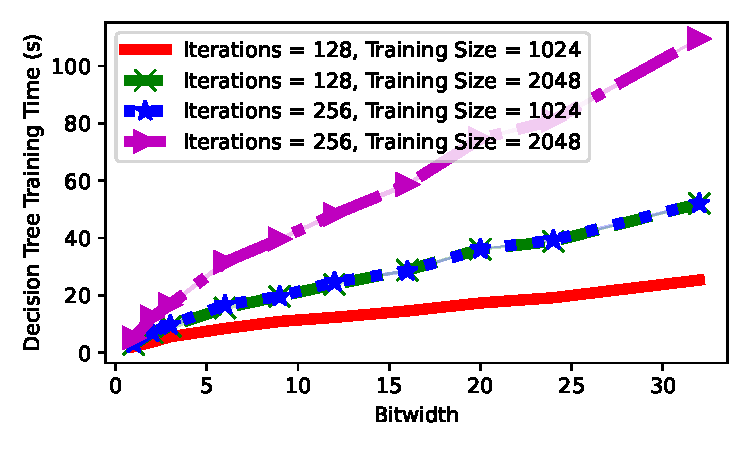
\includegraphics[width=\gsize]{graphs/time_beaver_triple_gen_beaver_256_2048.pdf} \\
    \hline
    \hline
\end{tabular}
\caption{Experimental results: decision tree training time.}
\label{fig:results_training_time}
\end{figure*}


% These are full figures for the appendix

\begin{figure*}
  \centering
  \newcommand{\gsize}{.45\textwidth}
\begin{tabular}{c| c c}
    \hline\hline
  & \textbf{OT-Based (GMW)} & \textbf{Beaver Triple-Based}\\
    \hline\hline
  \rotatebox{90}{\phantom{helloh}$i = 128, n = 1024$}
  & 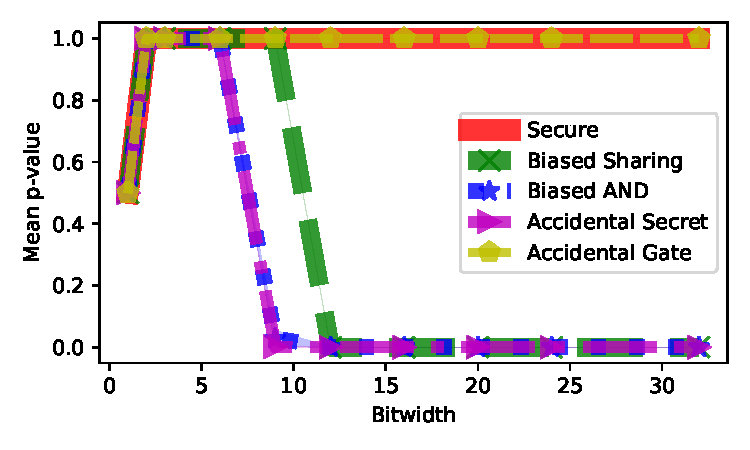
\includegraphics[width=\gsize]{graphs/security_adder_gmw_128_1024.pdf}
                 & 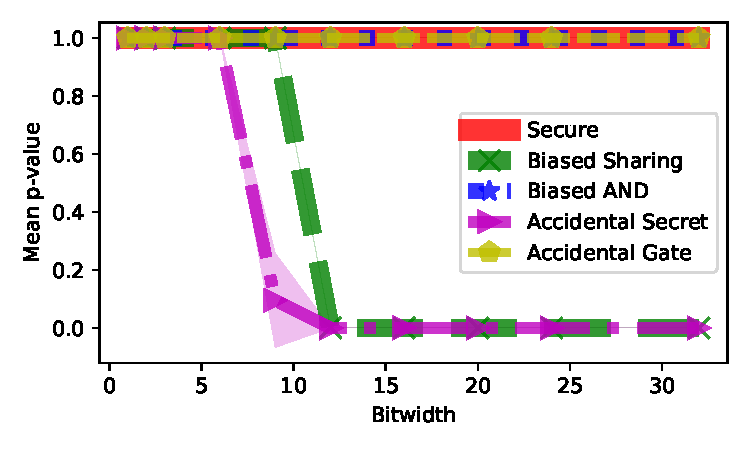
\includegraphics[width=\gsize]{graphs/security_adder_beaver_128_1024.pdf} \\
    \hline
  \rotatebox{90}{\phantom{helloh}$i = 128, n = 2048$}
  & 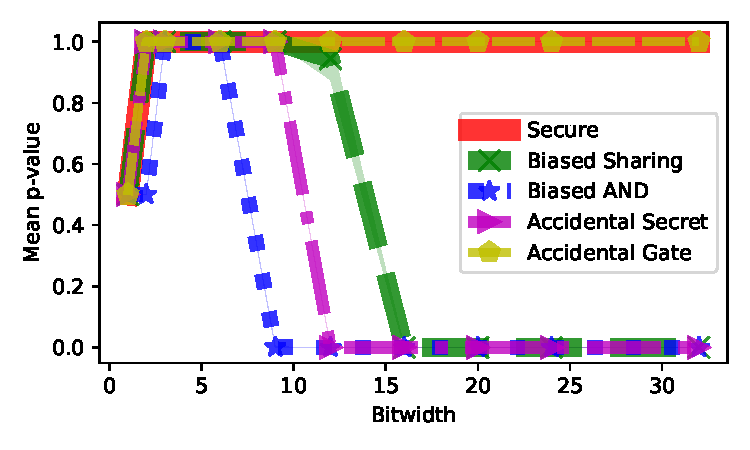
\includegraphics[width=\gsize]{graphs/security_adder_gmw_128_2048.pdf}
                 & 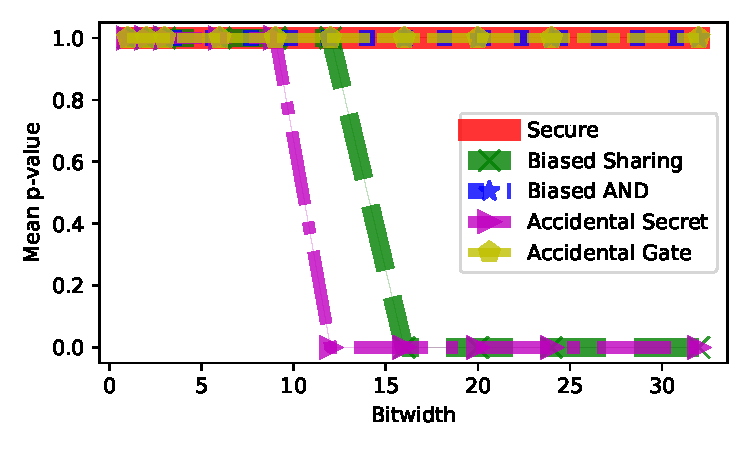
\includegraphics[width=\gsize]{graphs/security_adder_beaver_128_2048.pdf} \\
    \hline
  \rotatebox{90}{\phantom{helloh}$i = 256, n = 1024$}
  & 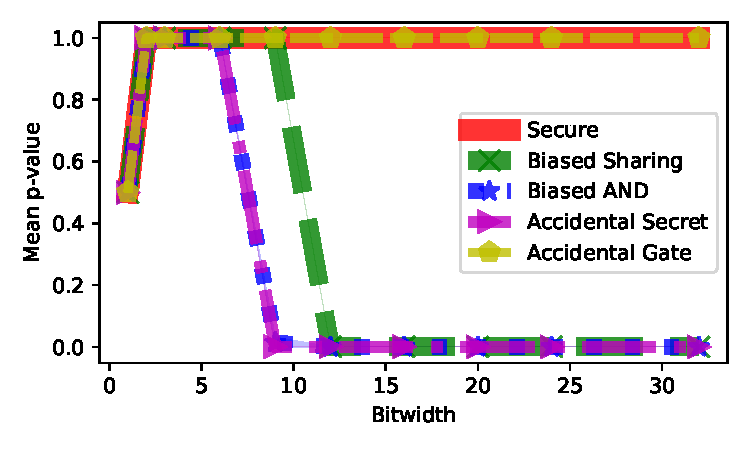
\includegraphics[width=\gsize]{graphs/security_adder_gmw_256_1024.pdf}
                 & 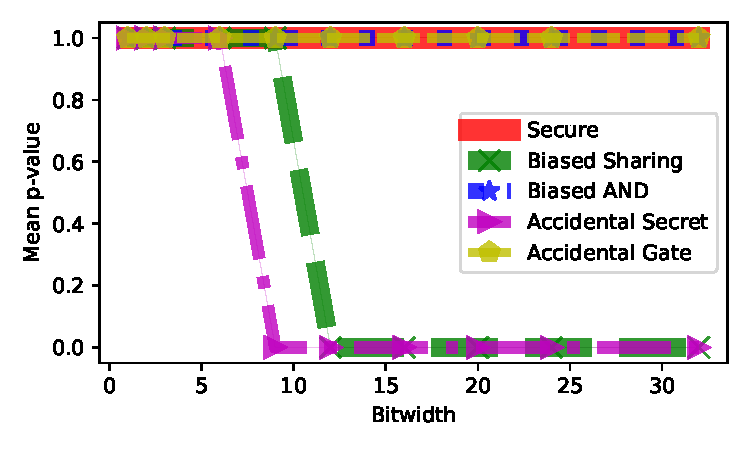
\includegraphics[width=\gsize]{graphs/security_adder_beaver_256_1024.pdf} \\
    \hline
  \rotatebox{90}{\phantom{helloh}$i = 256, n = 2048$}
  & 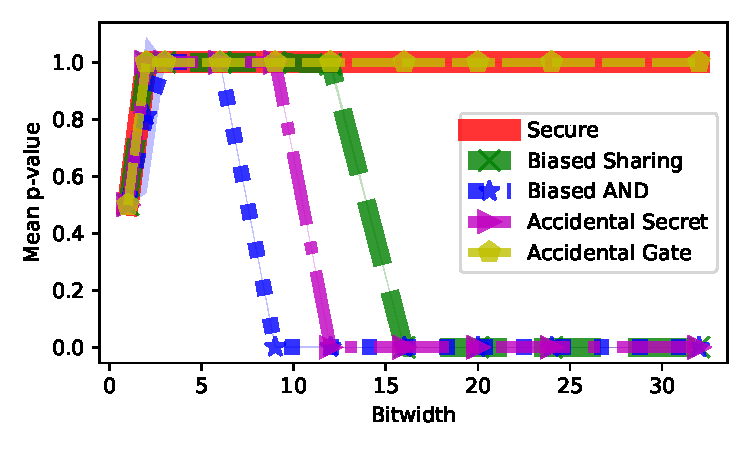
\includegraphics[width=\gsize]{graphs/security_adder_gmw_256_2048.pdf}
                 & 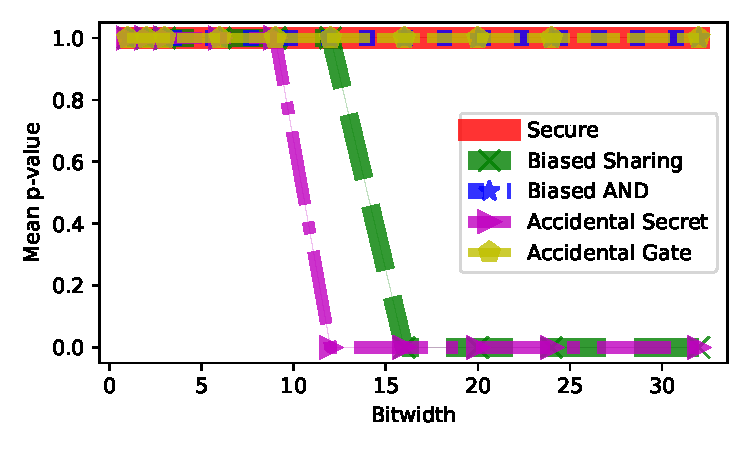
\includegraphics[width=\gsize]{graphs/security_adder_beaver_256_2048.pdf} \\
    \hline
    \hline
\end{tabular}
\caption{Experimental results, $n$-bit addition.}
\label{fig:extra1}
\end{figure*}

\begin{figure*}
  \centering
  \newcommand{\gsize}{.45\textwidth}
\begin{tabular}{c| c c}
    \hline\hline
  & \textbf{OT-Based (GMW)} & \textbf{Beaver Triple-Based}\\
    \hline\hline
  \rotatebox{90}{\phantom{helloh}$i = 128, n = 1024$}
  & 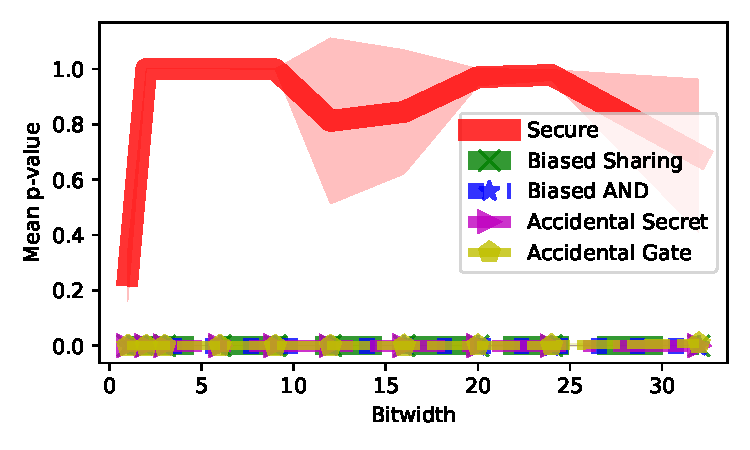
\includegraphics[width=\gsize]{graphs/security_less_than_gmw_128_1024.pdf}
                 & 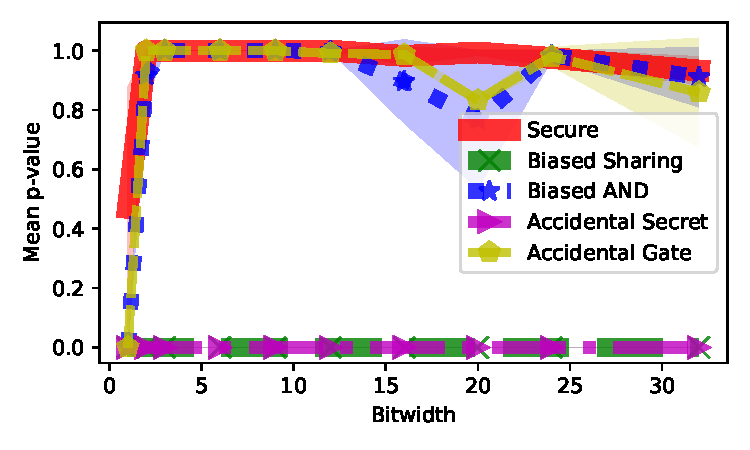
\includegraphics[width=\gsize]{graphs/security_less_than_beaver_128_1024.pdf} \\
    \hline
  \rotatebox{90}{\phantom{helloh}$i = 128, n = 2048$}
  & 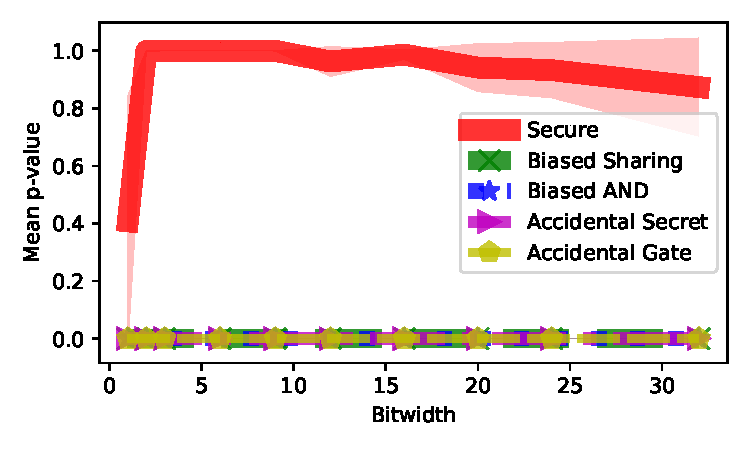
\includegraphics[width=\gsize]{graphs/security_less_than_gmw_128_2048.pdf}
                 & 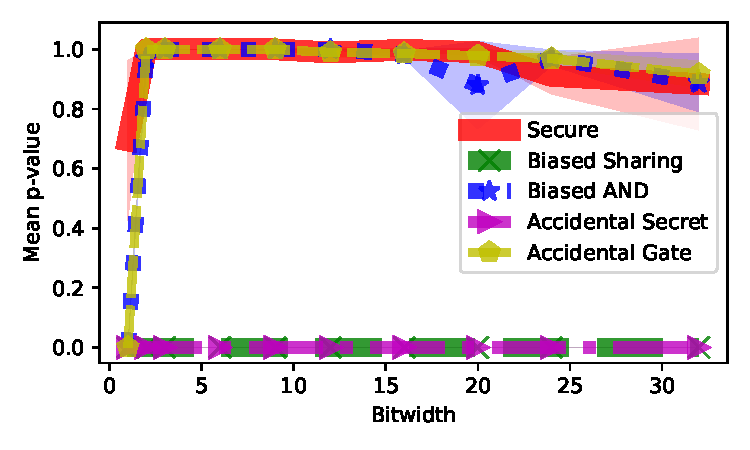
\includegraphics[width=\gsize]{graphs/security_less_than_beaver_128_2048.pdf} \\
    \hline
  \rotatebox{90}{\phantom{helloh}$i = 256, n = 1024$}
  & 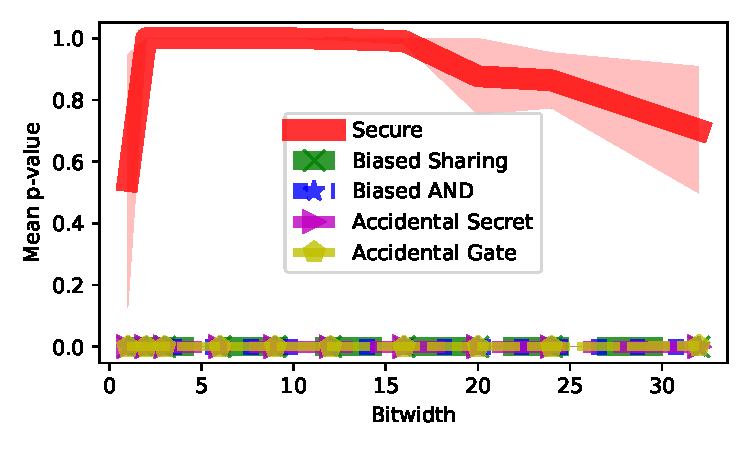
\includegraphics[width=\gsize]{graphs/security_less_than_gmw_256_1024.pdf}
                 & 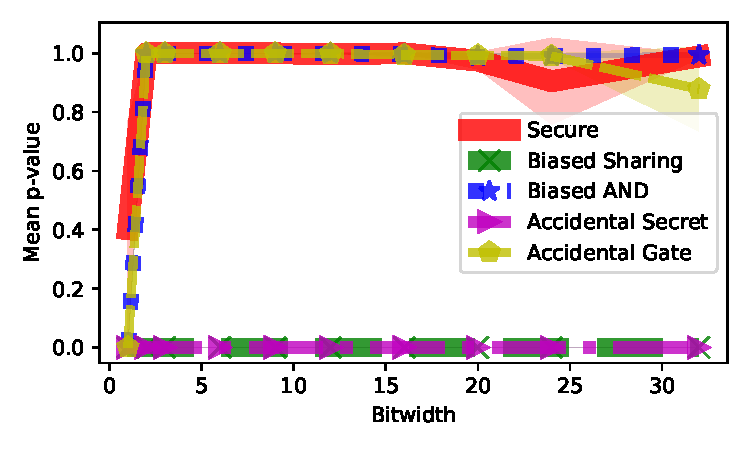
\includegraphics[width=\gsize]{graphs/security_less_than_beaver_256_1024.pdf} \\
    \hline
  \rotatebox{90}{\phantom{helloh}$i = 256, n = 2048$}
  & 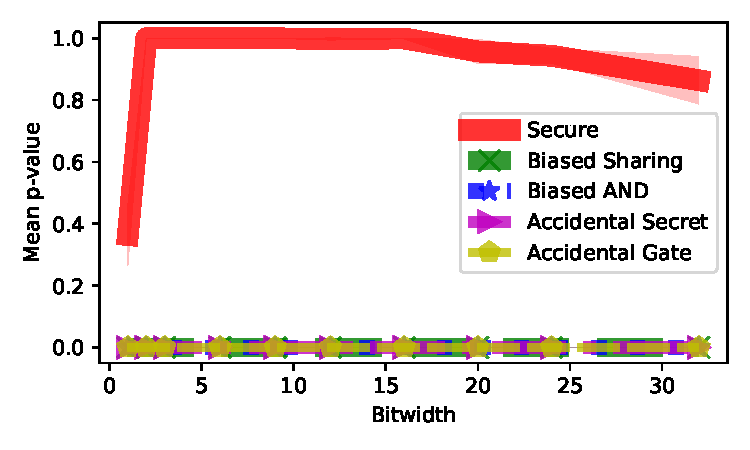
\includegraphics[width=\gsize]{graphs/security_less_than_gmw_256_2048.pdf}
                 & 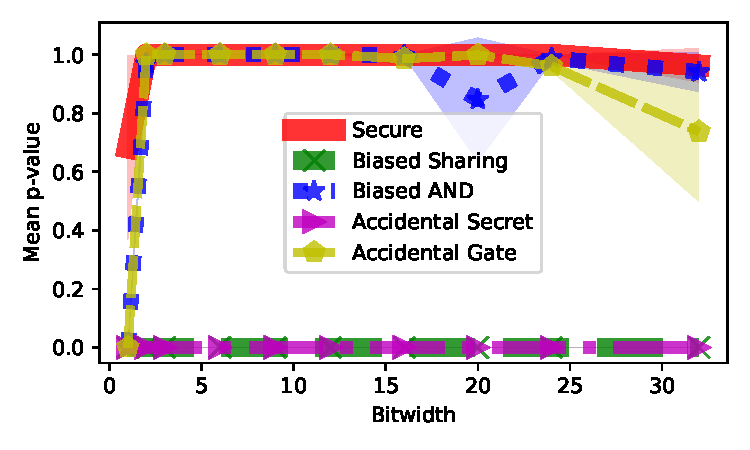
\includegraphics[width=\gsize]{graphs/security_less_than_beaver_256_2048.pdf} \\
    \hline
    \hline
\end{tabular}
\caption{Experimental results, $n$-bit less-than comparison.}
\label{fig:extra2}
\end{figure*}

\begin{figure*}
  \centering
  \newcommand{\gsize}{.45\textwidth}
\begin{tabular}{c| c c}
    \hline\hline
  & \textbf{OT-Based (GMW)} & \textbf{Beaver Triple-Based}\\
    \hline\hline
  \rotatebox{90}{\phantom{helloh}$i = 128, n = 1024$}
  & 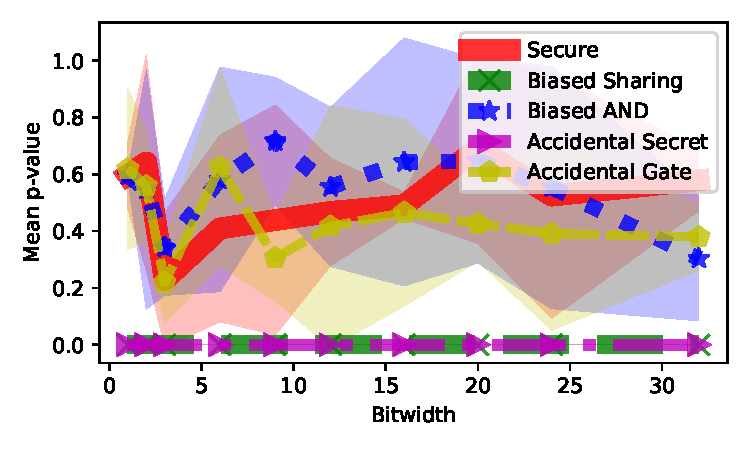
\includegraphics[width=\gsize]{graphs/security_beaver_triple_gen_gmw_128_1024.pdf}
                 & 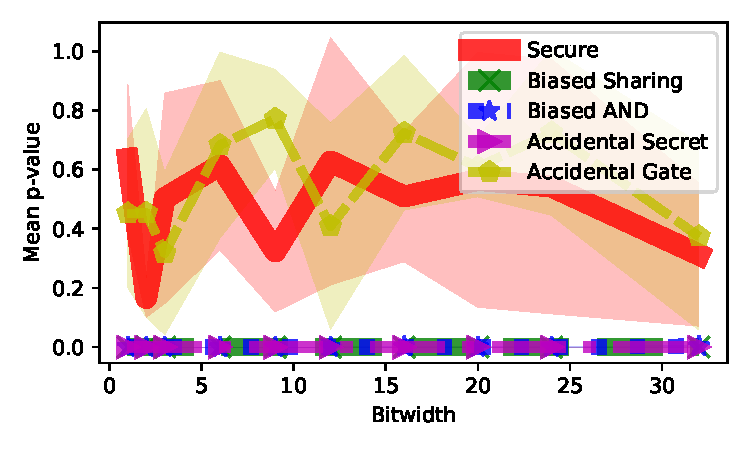
\includegraphics[width=\gsize]{graphs/security_beaver_triple_gen_beaver_128_1024.pdf} \\
    \hline
  \rotatebox{90}{\phantom{helloh}$i = 128, n = 2048$}
  & 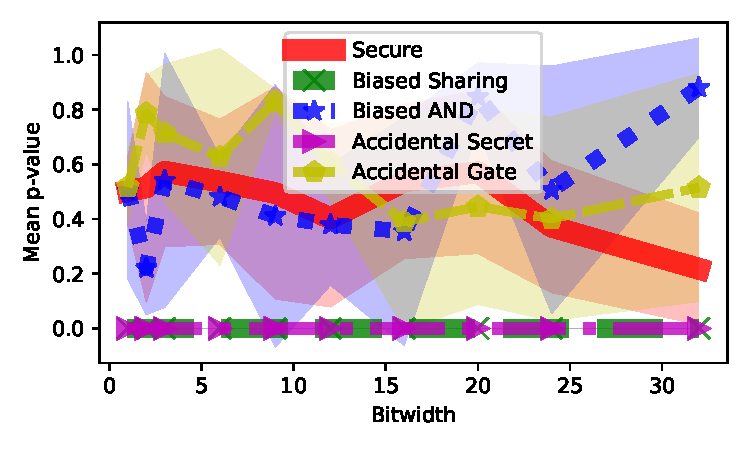
\includegraphics[width=\gsize]{graphs/security_beaver_triple_gen_gmw_128_2048.pdf}
                 & 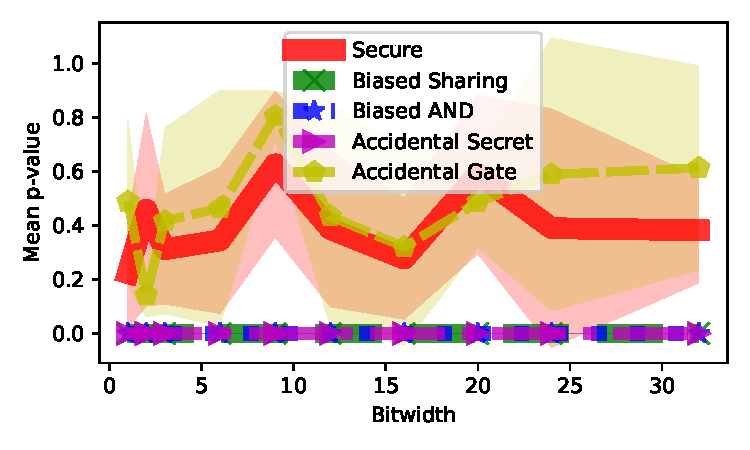
\includegraphics[width=\gsize]{graphs/security_beaver_triple_gen_beaver_128_2048.pdf} \\
    \hline
  \rotatebox{90}{\phantom{helloh}$i = 256, n = 1024$}
  & 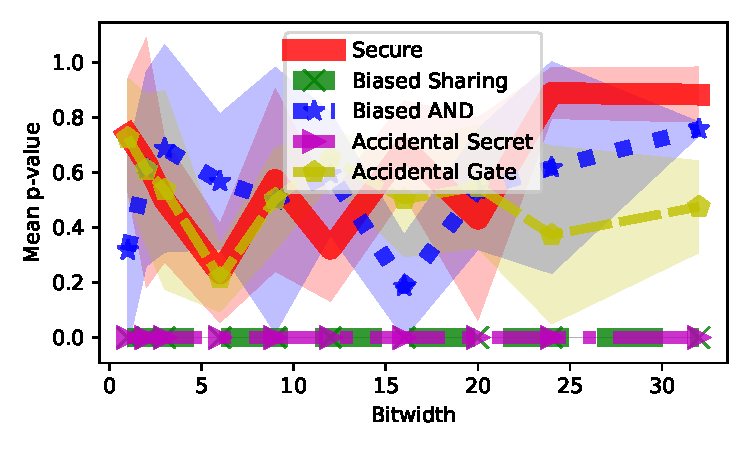
\includegraphics[width=\gsize]{graphs/security_beaver_triple_gen_gmw_256_1024.pdf}
                 & 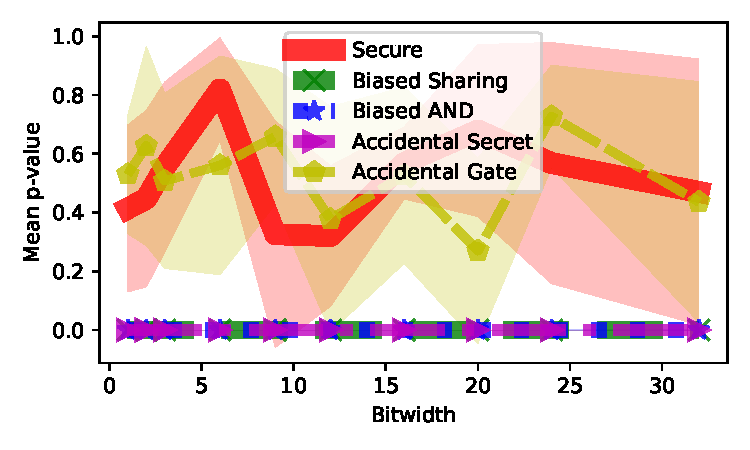
\includegraphics[width=\gsize]{graphs/security_beaver_triple_gen_beaver_256_1024.pdf} \\
    \hline
  \rotatebox{90}{\phantom{helloh}$i = 256, n = 2048$}
  & 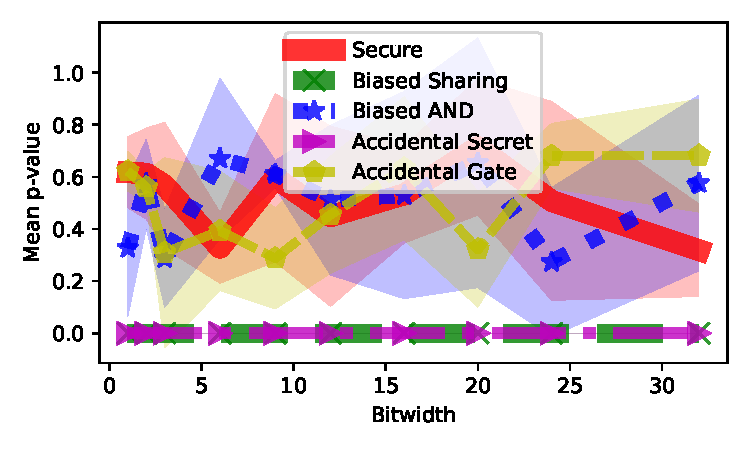
\includegraphics[width=\gsize]{graphs/security_beaver_triple_gen_gmw_256_2048.pdf}
                 & 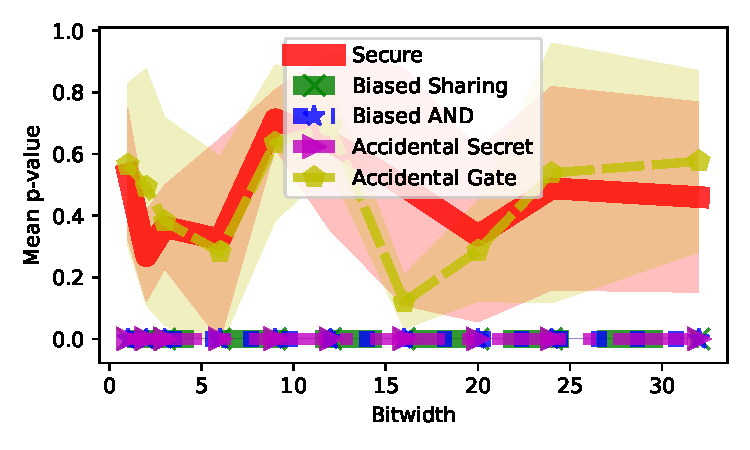
\includegraphics[width=\gsize]{graphs/security_beaver_triple_gen_beaver_256_2048.pdf} \\
    \hline
    \hline
\end{tabular}
\caption{Experimental results, $n$-bit Beaver triple generation.}
\label{fig:extra3}
\end{figure*}




\section{Example \langname program}\label{sec:example-big}

The following \langname uses oblivious-transfer based GMW to evaluate a circuit representing a "less than" function
between the two parties' inputs, interpreted as 2-bit binary numbers.
It is slightly shorter than the ones we used for our experiments;
to provide the closest possible comparison between different implementations in our experiments,
the \langname protocols we used included some "no-op" statements.

\begin{small}
\begin{verbatim}
-- two_bit_less_than.cho
MACRO secret_share(P1(x), P2()) AS
  s1 = FLIP @P1
  s2 = x + s1
  SEND s2 TO P2
ENDMACRO
MACRO and_gmw(P1(x2, y2), P2(x1, y1)) AS
  out2 = FLIP @P2
  g1_s2_00 = out2 + ((x1 + 0) ^ (y1 + 0))
  g1_s2_01 = out2 + ((x1 + 0) ^ (y1 + 1))
  g1_s2_10 = out2 + ((x1 + 1) ^ (y1 + 0))
  g1_s2_11 = out2 + ((x1 + 1) ^ (y1 + 1))
  out1 = OBLIVIOUSLY [[g1_s2_00,
                       g1_s2_01]?y2,
                      [g1_s2_10,
                       g1_s2_11]?y2
                     ]?x2 FOR P1
ENDMACRO
MACRO reveal(P1(x1), P2(x2)) AS
  SEND x1 TO P2
  SEND x2 TO P1
  y = x1 + x2
ENDMACRO
-- Read secrets
x0 = SECRET @P1
x1 = SECRET @P1
y2 = SECRET @P2
y3 = SECRET @P2
-- Set up shares
DO secret_share(P1(x0), P2()) GET(x0_1=s1,
                                  x0_2=s2)
DO secret_share(P1(x1), P2()) GET(x1_1=s1,
                                  x1_2=s2)
DO secret_share(P2(y2), P1()) GET(y2_1=s2,
                                  y2_2=s1)
DO secret_share(P2(y3), P1()) GET(y3_1=s2,
                                  y3_2=s1)
-- Circuit evaluation
g3_1 = ~y2_1
g3_2 = y2_2
DO and_gmw(P1(x0_1, g3_1), P2(x0_2, g3_2)
          ) GET(g4_1=out1, g4_2=out2)
g5_1 = ~x0_1
g5_2 = x0_2
DO and_gmw(P1(y2_1, g5_1), P2(y2_2, g5_2)
          ) GET(g6_1=out1, g6_2=out2)
g7_1 = ~y3_1
g7_2 = y3_2
g8_1 = ~g6_1
g8_2 = g6_2
DO and_gmw(P1(g7_1, g8_1), P2(g7_2, g8_2)
          ) GET(g9_1=out1, g9_2=out2)
DO and_gmw(P1(x1_1, g9_1), P2(x1_2, g9_2)
          ) GET(g10_1=out1, g10_2=out2)
DO and_gmw(P1(g4_1, g10_1), P2(g4_2, g10_2)
          ) GET(g11_1=out1, g11_2=out2)
g12_1 = g4_1 + g10_1
g12_2 = g4_2 + g10_2
g13_1 = g11_1 + g12_1
g13_2 = g11_2 + g12_2
-- Reveal output
DO reveal(P1(g13_1), P2(g13_2)) GET(r0=y)
OUTPUT r0
\end{verbatim}
\end{small}

\end{document}
\endinput
%%
%% End of file `sample-acmlarge.tex'.
